\documentclass[12pt]{report}

\usepackage[dutch]{babel}
\usepackage[nobottomtitles]{titlesec}
\usepackage[bottom]{footmisc}
\usepackage{graphicx}
\usepackage{titleps}
\usepackage{amssymb}
\usepackage{amsmath}
\usepackage{amsthm}
\usepackage{graphicx}
\usepackage{verbatim}
\usepackage{titling}
\usepackage[toc,page]{appendix}
\usepackage{bm}

\usepackage{fancyhdr}

\pagestyle{fancy}

\renewcommand{\chaptermark}[1]{\markboth{#1}{}}
\renewcommand{\sectionmark}[1]{\markright{#1}}
\fancyhf{}
\fancypagestyle{plain}{%
  \fancyhf{}%
	\rfoot{\fancyplain{}{\nouppercase{\thepage}}}
	\lfoot{\fancyplain{}{Thorvald Dox}}
  \renewcommand{\headrulewidth}{0pt}% Line at the header invisible
  \renewcommand{\footrulewidth}{0.4pt}% Line at the footer visible
}
\lhead{\fancyplain{}{Semilineaire MESMA}}
\rhead{\fancyplain{}{\nouppercase{\leftmark}}}
\rfoot{\fancyplain{}{\nouppercase{\thepage}}}
\lfoot{\fancyplain{}{Thorvald Dox}}
\renewcommand{\footrulewidth}{0.4pt}

\fancyhfoffset[E,O]{0pt}
\date{}
  
\usepackage[margin=1in]{geometry}
\usepackage{float}



\usepackage[super,sort]{natbib}
\usepackage{bibentry}
\nobibliography*

\newcommand{\footcite}[1]{\cite{#1}\let\thefootnote\relax \footnote{\cite{#1} \bibentry{#1}} }

\DeclareMathOperator*{\Odot}{\bigodot}
\allowdisplaybreaks

%\title{Semi-lineair Multiple Endmember mixture spectrum analysis}
\title{Semilineaire spectraalanalyse met meerdere eindmembers}
\author{Thorvald Dox}

\begin{document}
\begin{titlepage}

\newcommand{\HRule}{\rule{\linewidth}{0.5mm}} % Defines a new command for the horizontal lines, change thickness here

\center % Center everything on the page
 
%----------------------------------------------------------------------------------------
%	HEADING SECTIONS
%----------------------------------------------------------------------------------------

\textsc{\LARGE Universiteit Antwerpen}\\[1.5cm] % Name of your university/college
\textsc{\Large Fysica}\\[0.5cm] % Major heading such as course name
\textsc{\large Masterproef}\\[0.5cm] % Minor heading such as course title

%----------------------------------------------------------------------------------------
%	TITLE SECTION
%----------------------------------------------------------------------------------------

\HRule \\[0.4cm]
{ \Large \bfseries \thetitle}\\[0.4cm] % Title of your document
\HRule \\[1.5cm]
 
%----------------------------------------------------------------------------------------
%	AUTHOR SECTION
%----------------------------------------------------------------------------------------

\begin{minipage}{0.4\textwidth}
\begin{flushleft} \large
\emph{Auteur:}\\
\theauthor % Your name
~\\
~\\
~\\
\end{flushleft}
\end{minipage}
~
\begin{minipage}{0.4\textwidth}
\begin{flushright} \large
\emph{Promotor:} \\
Paul {Scheunders} \\ % Supervisor's Name
\emph{Copromotor:} \\
Rob {Heylen} % Supervisor's Name
\end{flushright}
\end{minipage}\\[5cm]

% If you don't want a supervisor, uncomment the two lines below and remove the section above
%\Large \emph{Author:}\\
%John \textsc{Smith}\\[3cm] % Your name

%----------------------------------------------------------------------------------------
%	DATE SECTION
%----------------------------------------------------------------------------------------

%{\large \today}\\[3cm] % Date, change the \today to a set date if you want to be precise

%----------------------------------------------------------------------------------------
%	LOGO SECTION
%----------------------------------------------------------------------------------------

%
\includegraphics[height=4cm]{remote.png}

\includegraphics[height=4cm]{download.jpg}
\hspace{5 cm}

\includegraphics[height=4cm]{vlabsym.png}
 \\[1cm] % Include a department/university logo - this will require the graphicx package

 
%----------------------------------------------------------------------------------------

\vfill % Fill the rest of the page with whitespace

\end{titlepage}
\tableofcontents
\newpage
\chapter*{Abstract}
\addcontentsline{toc}{chapter}{Abstract}

\newpage
\chapter*{Inleiding}
\addcontentsline{toc}{chapter}{Inleiding}

%TODO het belang van aardopservatie
Hyperspectrale ontmenging heeft toepassingen in voedselveiligheid, farmaceutische proces- en kwaliteitscontrole, en andere medische, biomedische, biometrische, industri\"ele en forensische toepassingen\footcite{dias12}. Maar een van de belangrijkste toepassingen in aardobservatie. Aardobservatie hoeft niet altijd op de aarde te slaan, dit kan ook gebruikt worden op andere planeten, maar het vaakst worden deze gebruikt om satellietbeelden van de aarde te interpreteren. Deze kunnen gebruikt worden om effectief gebieden in kaart te brengen, tot in groot detail. Er kan bijvoorbeeld de groei van een invasieve soort plant in kaart worden gebracht, zelfs als die voor ons menselijk oog erg lijkt op een andere inheemse plant. Ook kunnen bijvoorbeeld op het oppervlak van de aarde of andere planeten zoals Mars de verschillende soorten gesteenten in kaart worden gebracht, zonder dat iemand letterlijk in de buurt moet komen van deze gesteenten of een monster moet bestuderen in een laboratorium.

Een van de grote problemen van het interpreteren van data is het omzetten van een beeld, dat spectra bevat, naar een kaart die de materialen weergeeft. Dit is een van de problemen die worden opgelost door het zogenaamde ontmengen.

Voor de werkelijke implementatie van de in dit verslag beschreven algoritmen wordt gebruikt gemaakt van \textit{matlab}\footcite{MATLAB}. De code kan gevonden worden op \\ \textit{https://github.com/thorvalddox/Hyperspectral}.

\chapter{Ontmengen}

\section{Het begrip spectrum}

%TODO herschrijf

Een spectrum is een eigenschap van licht. Het bevat de intensiteit van een lichtstraal in functie van de golflengte of frequentie. Dit spectrum kan gemeten worden door de zogenaamde hyperspectrale camera's, die dit spectrum voor elke pixel opmeten. Aangezien deze maar op een aantal discrete golflengten meten en niet over het hele oneindige spectrum, is het resultaat in praktijk geen functie, maar gewoon een numerieke vector van data.

\section{Het begrip ontmengen}

Als een hyperspectrale camera een afbeelding neemt van bijvoorbeeld het aardoppervlak, beschrijft een enkele pixel een gebied waarin zich meerdere materialen bevinden. Dit is altijd het geval, onafhankelijk van de resolutie van de camera\footcite{dias12}. Neem bijvoorbeeld een bos. Als de pixels groter zijn dan een vierkante meter staan verschillende soorten bomen op eenzelfde pixel. Als de pixels kleiner worden kunnen we deze wel onderscheiden, maar dan kunnen de takken nog niet van de bladeren onderscheiden worden. Zelfs als we elk blad afzonderlijk kunnen onderscheiden, de nerven van het blad hebben een ander spectrum dan het bladmoes. Zelf als we verder inzoomen, de cellen van het blad bestaan nog altijd uit verschillende materialen. Bijvoorbeeld bij een gesteente, dat bestaat uit verschillende mineralen, maakt het niet uit hoe ver er ingezoomd wordt, de mineralen blijven vermengd tot op atomair niveau.

Hierom is het belangrijk een manier te vinden om de verschillende materialen uit een pixel te ``ontmengen''. Dit wil zeggen dat uit een spectrum van de volledige pixel de ``hoeveelheden'' en de spectra van de verschillende materialen afgeleid kan worden. Dit proces heet ontmengen.

Het is belangrijk om in te zien dat een materiaal ofwel eindmember genoemd niet per definitie een enkele moleculair zuivere stof moet zijn. In het bovenstaande voorbeeld zullen waarschijnlijk de verschillende bladeren van eenzelfde boom -of zelfs de hele boom of, wat meestal gebruikt wordt, alle bomen - als een enkele eindmember beschouwd worden.


\section{Lineair model}
In het lineaire model gaan we ervan uit dat het gemeten spectrum een lineaire combinatie is van de spectra van de verschillende eindmembers. De voorfactoren geven de ``hoeveelheid'' weer van een materiaal dat zich bevindt in het spectrum, deze voorfactoren noemen we abundanties. De spectra in dit model kunnen ontmengd worden door gebruik te maken van onder andere ``sum-to-one constrained least square unmixing''\footcite{mesma}, wat in dit verslag gebruikt wordt. Dit zoekt de set van abundacies met de laagste Gaussische reconstructie-error. De reconstructie-error is de kwadratische norm van het verschil van het werkelijke spectrum, en het spectrum dat ontstaat door het model te mengen met de set gevonden eindmembers en parameters. In het lineaire model kan het minimum gevonden worden door het gemeten spectrum te projecteren op het hypervlak, opgespannen door de eindmembers.

Noemen we de reflectiespectra van de verschillende eindmembers $\bm{e}_i$, de respectievelijke abundanties $a_i$ en de ruis $\eta$, dan is het totale reflectiespectrum gelijk aan\footcite{mesma}:

\begin{align}
\bm{x} &= \sum_i a_i \bm{e}_i + \eta
\end{align}

In een experiment zijn $\bm{x}$ en $\bm{e}_i$ gekend, maar $a_i$ en $\eta$ niet. Sterker nog, aangezien de ruis klein is, is men ge\"intereseerd in de abundanties waarvoor de ruis het kleinst is, of specifieker, waar de kwadratische norm van de ruis het kleinst is. Dit komt overeen met de minimale Gaussische afstand te zoeken tot het hypervlak, opgespannen door de eindmembers. Dit is equivalent met het systeem projecteren op het hypervlak. %TODO fix zin

\begin{align}
\text{argmin}_{a_1 ... a_p} \left| \bm{x} - \sum_{i=1}^p a_i \bm{e}_i\right|^2
\end{align}

Hierbij is $p$ het totaal aantal eindmembers.


\subsubsection{Sommeer tot een}

Als extra voorwaarde wordt opgelegd dat de som van de verschillende abundanties gelijk aan een is. Dit kan gedaan worden als hierna beschreven. 

De volledige hyperruimte wordt getranslateerd volgens een van de eindmembers, $\bm{e}_1$. Hierdoor is de hyperruimte opgespannen door de eindmembers een deelruimte, en kan er dus op geprojecteerd worden door middel van Penrose- inversen \footcite{mesma}. De waarde van het totale spectrum en de eindmembers worden in de nieuwe hyperruimte respectievelijk $\bm{x} - \bm{e}_1$ en $\bm{e}_i - \bm{e}_1$. Als $J$ de matrix is gedefinieerd door de vectoren $\bm{e}_i - \bm{e}_1$ voor $i$ van $2$ tot $p$ als kolommen aan elkaar te rijgen, dan geldt:

\begin{equation}
\hat{a} = \left(J^T J\right)^{-1} J^T \bm{x}
\end{equation} 

met $\hat{a}$ de kolommatrix met de abundanties. Deze bevat nog niet de abundantie van $\bm{e}_1$, maar deze kan gevonden worden dankzij de voorwaarde dat de som een is, zodat $a_1 = 1 - \sum_{i=2}^{p} a_i$.

\subsubsection{Niet-negativiteitsvoorwaarde}

Een andere extra voorwaarde is dat de abundanties niet negatief mogen zijn. Dit kan verwezenlijkt worden door in plaats van Penrose-Inversie een niet-negativiteitsalgoritme te gebruiken, maar later in deze thesis zal dit verwezenlijkt worden op een andere manier.
%\section{Pixel purity}


\chapter{Multilinear model}\label{mlm}


Het multilineair model\footcite{mlinmix} is een model dat oneindig veel ordes meeneemt, door de interactie van licht met de materialen op het monster te modelleren als een discreet Markov-proces. Deze bevat de volgende stappen, zoals beschreven in \textit{A multilinear mixing model for nonlinear spectral unmixing}\footcite{mlinmix}.
\begin{enumerate}
\item De inkomende straal interageert met minstens \'e\'en materiaal in de bron.
\item Na deze interactie heeft het materiaal een kans $P$ om een nieuwe interactie aan te gaan, en een kans $(1-P)$ om dat niet te doen.
\item De kans om een nieuwe interactie aan te gaan met elk nieuw materiaal is evenredig met de abundantie van dat materiaal. Merk op dat aangezien de som van de abundaties \'e\'en is, de waarde van de kans gelijk is aan de abundantie.
\item Wanneer een lichtstraal interageert met een materiaal wordt zijn spectrum gewijzigd, afhankelijk van het albedo van dit materiaal.
\end{enumerate}

De interactie van dit materiaal verloopt als volgt:
\begin{equation}
\bm{x}' = \bm{w} \odot \bm{x}
\end{equation}
waarbij $\bm{x}'$ de uitgaande straal is, $\bm{w}$ het albedo is, $\bm{x}$ de inkomende straal en $\odot$ het Hadamard product, ofwel elementgewijs product wat gedefinieerd is als volgt:
\begin{equation}
\left(\bm{x} \odot \bm{y}\right)_i = x_i.y_i
\end{equation}



\section{Berekening}

In deze sectie gaan we uit van een homogene lichtbron. In sectie \ref{sec:at_cor} wordt deze eis versoepeld.

De kans dat een welbepaald pad gevolgd wordt, wordt als volgt genoteerd:

\begin{equation}
\mathcal{P}(i_1,i_2,i_3,...,i_R)
\end{equation}

Bovenstaande uitdrukking geeft de kans dat een lichtstraal respectievelijk reflecteert op materiaal 
$i_1$,$i_2$,$i_3$ en zo voort. $R$ is hier het totale aantal materialen waarop gereflecteerd wordt.

Deze kan aan de hand van het voorgaande Markov-proces berekend worden\footcite{mlinmix}. 

\begin{equation}
\mathcal{P}(i_1,i_2,i_3,...,i_R) = P^{R-1} (1-P) \prod_{k=1}^R a_{i_k}
\end{equation}

De uitgaande straal ten gevolge van een specifiek pad is 
$\Odot_{k=1}^R \bm{w}_{i_k}$ dus is de kans op de uitgaande straal vermenigvuldigd met het spectrum:
\begin{equation}
\bm{x}_{(i_1,i_2,i_3,...,i_R)} = P^{R-1} (1-P) \Odot_{k=1}^R \left(a_{i_k} \bm{w}_{i_k}\right)
\end{equation}

We noemen dit de amplitudo van dit pad.

Gesommeerd over alle mogelijke paden wordt dit:

\begin{equation}
\bm{x} = \sum_{R=1}^{\infty} \left(\sum_{i_1}^{p} ... \sum_{i_R}^{p}\right)P^{R-1} (1-P) \Odot_{k=1}^R \left(a_{i_k} \bm{w}_{i_k}\right)
\end{equation}

\section{Atmosferische correctie} \label{sec:at_cor}

De lichtbron die we gebruiken om ons monster te belichten, is in de meeste gevallen de zon. Bij lineaire ontmenging, waarbij we ge\"intereseerd waren in reflectiespectra, gaf deze gewoon een lineaire factor waarmee alle reflectiespectra vermenigvuldigd waren. Als alle eindmembers ook hiermee vermenigvuldigd worden, geeft deze dankzij het lineaire karakter van het systeem het juiste resultaat.

Dit is niet meer het geval bij multilineair ontmengen, aangezien we werken met albedo's in plaats van reflectiespectra. Als we het spectrum van de lichtbron $\bm{I}$ noemen, geldt dat 
\begin{equation}
\bm{x} = \sum_{R=1}^{\infty} \left(\sum_{i_1}^{p} ... \sum_{i_R}^{p}\right)P^{R-1} (1-P) \bm{I}\odot\Odot_{k=1}^R \left(a_{i_k} \bm{w}_{i_k}\right)
\end{equation}

Er bestaan vele technieken om dit probleem op te lossen, die ook rekening houden met de verschillende effecten van de atmosfeer. De datasets die in deze thesis gebruikt worden zijn al verwerkt door een dergelijk algoritme. 


\subsection{Schaduw}

Een pixel bevat een schaduw wanneer er minder licht invalt. Dit kan niet worden weggewerkt met bovenstaande methode omdat deze aanneemt dat het spectrum van het invallend licht overal gelijk is.
In dit geval hebben een aantal pixels een lichtbron met een andere intensiteit. Dit spectrum heeft dezelfde vorm als de oorspronkelijke lichtbron, alleen een kleinere intensiteit. Dit kan dus worden voorgesteld als een extra factor die toegevoegd wordt aan het systeem. We noteren deze $l$. De vergelijking wordt nu:

\begin{equation}
\bm{x} = l\sum_{R=1}^{\infty} \left(\sum_{i_1}^{p} ... \sum_{i_R}^{p}\right)P^{R-1} (1-P) \bm{I}\odot\Odot_{k=1}^R \left(a_{i_k} \bm{w}_{i_k}\right)
\end{equation}

\section{Afhankelijke kansen} \label{sec:Pi}

Stel dat de kans dat een lichtstraal nog een keer interageert afhankelijk is van het materiaal. Dit kan voorkomen bij bijvoorbeeld een zandgrond met vegetatie erboven. Een lichtstraal die vertrekt op de grond zal met een grotere waarschijnlijkheid eerst met de vegetatie erboven interageren voor het op de detector terecht komt.

\begin{align}
\mathcal{P}(i_1,i_2,i_3,...,i_R) &= \prod_{k=1}^{R-1}P_{i_k} (1-P_{i_R})\\
&= \prod_{k=1}^{R}P_{i_k} \frac{1-P_{i_R}}{P_{i_R}}
\end{align}


%Nu, laten we de verzameling beschouwen van alle mogelijke paden $(i_1,i_2,i_3,...,i_R)$. Deze kan worden verdeeld in klassen, waarbij elementen in dezelfde klasse worden geplaatst als ze een permutatie zijn van elkaar. Bijvoorbeeld $(1,2,3)$, $(2,1,3)$ en $(3,2,1)$ zitten in dezelfde klassen, maar $(1,2)$,$(1,2,3,4)$ en $(3,4,5)$ zitten allemaal in een verschillende klasse. Als we de $\mathcal{P}$ waarde van elk pad vervangen door het gemiddelde uit zijn klasse, die we $\mathcal{P'}$ zullen noemen, dan blijft de som over de reflectiespectr over alle paden gelijk. Merk op dt dit niet in het algemeen het geval is, maar alleen omdat de paden in eenzelfde klasse hetzelfde reflectiespectrum hebben.
%
%\begin{align}
%\mathcal{P'}(i_1,i_2,i_3,...,i_R) &= \prod_{k=1}^{R}P_{i_k} \frac{1}{R}\sum_{k=1}^{R}\frac{1-P_k}{P_k}
%\end{align}
%
%Veronderstel dat de verschillende $P_i$ waarden bij benadering aan elkaar gelijk zijn. Dit is niet zo een onverwachte eis, aangezien voordien deze waarden exact gelijk werden verondersteld. Met bij benadering gelijk bedoelen we dat $\forall i,j: \frac{P_i}{P_j} \approx 1$ en $\frac{1 - P_i}{1 - P_j} \approx 1$. Dus 0.51 en 0.52 zijn ongeveer gelijk, maar 0.001 en 0.000001 niet, hoewel de laatste twee getallen een veel kleiner verschil hebben. Dan kan het rekenkundig gemiddelde $\sum_{k=1}^{R}\frac{1-P_k}{P_k}$ vervangen worden door het meetkundig gemiddelde $\sqrt[R]{\prod_{k=1}^{R}\frac{1-P_k}{P_k}}
%

De amplitudo van dit pad wordt:

\begin{align}
\bm{x}_{(i_1,i_2,i_3,...,i_R)} &= \prod_{k=1}^{R-1}P_{i_k} (1-P_{i_R}) \Odot_{k=1}^R \left(a_{i_k} \bm{w}_{i_k}\right) \\
&= \Odot_{k=1}^{R-1} \left(P_{i_k}a_{i_k} \bm{w}_{i_k}\right) \odot (1-P_{i_R}) a_{i_R} \bm{w}_{i_R} \\
\bm{x} &= \sum_{R=1}^{\infty} \left(\sum_{i_1}^{p} ... \sum_{i_R}^{p}\right) \Odot_{k=1}^{R-1} \left(P_{i_k}a_{i_k} \bm{w}_{i_k}\right) \odot (1-P_{i_R}) a_{i_R} \bm{w}_{i_R} \\
&= \sum_{i=1}^p (1-P_i) a_{i} \bm{w}_{i} + \sum_{i=1}^p \sum_{j=1}^p (1-P_i) a_{i} \bm{w}_{i} \odot P_j a_{j} \bm{w}_{j} \nonumber\\&+ \sum_{i=1}^p \sum_{j=1}^p \sum_{k=1}^p (1-P_i) a_{i} \bm{w}_{i} \odot P_j a_{j} \bm{w}_{j} \odot P_k a_{k} \bm{w}_{k} \nonumber\\&+ \sum_{i=1}^p \sum_{j=1}^p \sum_{k=1}^p  \sum_{l=1}^p (1-P_i) a_{i} \bm{w}_{i} \odot P_j a_{j} \bm{w}_{j} \odot P_k a_{k} \bm{w}_{k} \odot P_l a_{l} \bm{w}_{l} \nonumber \\& + ... \\
&= \bm{z} + \bm{y}\odot\bm{z} + \bm{y}\odot\bm{y}\odot\bm{z} + ... \\
&= \bm{z} + \bm{y}\odot\bm{x} \\
 &= \frac{\bm{z}}{1-\bm{y}}
\end{align}
waar
\begin{align}
\bm{y} &= \sum_{i=1}^p P_i a_{i} \bm{w}_{i} \\
\bm{z} &= \sum_{i=1}^p (1-P_i) a_{i} \bm{w}_{i} 
\end{align}
zodat
\begin{equation}
\bm{x} = \frac{\sum_{i=1}^p (1-P_i) a_{i} \bm{w}_{i}}{1-\sum_{i=1}^p P_i a_{i} \bm{w}_{i}} \label{eq:Pi}
\end{equation}
De vrijheidsgraden naar waar dit moet worden opgelost zijn $a_i$ en $P_i$, maar als volgende variabelen ingevoerd worden:
\begin{align}
b_i &= (1-P_i) a_i\\
c_i &= P_i a_i
\end{align}
ofwel 
\begin{align}
a_i &= b_i + c_i\\
P_i &= \frac{c_i}{b_i + c_i}
\end{align}
kan er geminimaliseerd worden naar $b_i$ en $c_i$.

Merk op dat $b_i$ en $c_i$ ook een fysische betekenis hebben. Als een lichtstraal op een pixel valt is
$a_i$ de kans dat deze lichtstraal op materiaal $i$ valt, is $b_i$ de kans dat deze op het materiaal valt en daarna als deze reflecteert op de detector valt en $c_i$ is de kans dat deze op het materiaal valt en reflecteert naar een ander materiaal. En de voorwaarde dat $\sum a_i = 1$ wordt nu $\sum b_i+c_i = 1$

\begin{equation} \label{eq:Pi}
\bm{x} = \frac{\sum_{i=1}^p b_{i} \bm{w}_{i}}{1-\sum_{i=1}^p c_{i} \bm{w}_{i}}
\end{equation}

Rekening houdend met errors moet de volgende vergelijking geminimaliseerd worden:

\begin{equation}
\text{min}_{b_i,c_i} \left\lVert \bm{x} - \frac{\sum_{i=1}^p b_{i} \bm{w}_{i}}{1-\sum_{i=1}^p c_{i} \bm{w}_{i}} \right\rVert^2 \label{eq:mlm}
\end{equation}

Hoe van dit systeem over te gaan naar het voorgaande systeem staat beschreven in sectie \ref{sec:P}

\subsection{Schaduw}

Als we schaduw terug toevoegen aan het systeem krijgen we

\begin{equation} \label{eq:Pi}
\bm{x} = \frac{l\sum_{i=1}^p b_{i} \bm{w}_{i}}{1-\sum_{i=1}^p c_{i} \bm{w}_{i}}
\end{equation}

Stel
\begin{equation}
b'_i = lb_i
\end{equation}
en stel
\begin{equation}
s = l^{-1}
\end{equation}



dan wordt de vergelijking hetzelfde als vergelijking \ref{eq:Pi}. Alleen vervalt de voorwaarde $\sum b'_i + c_i = 1$. Als alle $b'_i$'s en $c_i$'s bekend zijn, kan $s$ bepaald worden als volgt:

\begin{align}
\sum_i \left(b_i + c_i\right) &= 1 \\
\sum_i \left(sb'_i + c_i\right) &= 1 \\
s\sum_i b'_i + \sum_i c_i &= 1 \\
s = \frac{1-\sum c_i}{\sum_i b'_i} 
\end{align}

Bijgevolg is:

\begin{align}
a_i &= b_i + c_i \\
&= sb'_i + c_i \\
&= b'_i \frac{1-\sum c_i}{\sum_i b'_i} +c_i \\
\end{align}

Het is eenvoudig in te zien dat deze tot \'e\'en sommeren.



\subsection{Onafhankelijke kans} \label{sec:P}

In sectie \ref{sec:Pi} staat beschreven hoe men een systeem ontmengd gebruik makend van een verschillende reflectiekans voor elk materiaal. Als er uitgegaan wordt van een gelijke reflectiekans voor elk materiaal kan in formule \ref{eq:Pi} ge\"eist worden dat alle $P_i$ gelijk zijn. Dan vindt men volgende formule die ook gevonden werd in \textit{A multilinear mixing model for nonlinear spectral unmixing}\footcite{mlinmix}.

\begin{equation}
\bm{x} = \frac{(1-P)\sum_{i=1}^p  a_{i} \bm{w}_{i}}{1-P\sum_{i=1}^p  a_{i} \bm{w}_{i}} 
\end{equation}

Stel dat men het minimalisatie probleem heeft opgelost en een stel $P_i$'s en $a_i$'s gevonden heeft,
dan vindt men goede waarden voor $P$ en $a_i$ voor bovenstaand model. Het is logisch om te veronderstellen dat de $a_i$ voor beide systemen gelijk zijn, dit is echter niet altijd het geval. Wanneer een bepaald materiaal een hoge of lage $P_i$-waarde heeft in vergelijking met $P$, kan het zijn dat de abundantie in het minimum verschillend is. Maar laten we veronderstellen dat de abundanties voor beide systemen gelijk zijn.

Noem $P_i$ de kans dat een willekeurige straal als laatste ge\"interageerd heeft met materiaal $i$, gegeven dat het ge\"interageerd heeft ergens in de pixel. Dit is equivalent aan te stellen: hoe groot is de kans dat een willekeurige straal interageert met het specifieke materiaal $i$, gegeven dat het interageert met een willekeurig materiaal in de pixel? Uit sectie \ref{mlm} volgt dat dit de abundantie van het materiaal is en dat deze onafhankelijk is van de oorsprong van de lichtstraal. Wat is de kans dat deze lichtstraal afkomstig van materiaal $i$ nog een keer interageert met het materiaal. Deze was gegeven als $P_i$. Dit maakt de totale kans dat een lichtstraal nog eens interageert met het materiaal $\sum P_i a_i$. Dit is per definitie $P$, dus $P = \sum P_i a_i = \sum c_i$.


\subsection{Implementatie in matlab}

In matlab\footcite{MATLAB:2010} wordt vergelijking \ref{eq:mlm} geminimaliseerd aan de hand van de matlabfunctie \texttt{fmincon}, die deze functie numeriek minimaliseert.

Als dit ge\"implementeerd wordt kan er gebruik gemaakt worden van afhankelijke of onafhankelijke $P$ waarden, en kan schaduw wel of niet meegenomen worden. Als de kansen onafhankelijk zijn moet tussen het minimaliseren en de berekening van de abundanties, reflectie en reconstructie-error, $b$ en $c$ vervangen worden door

\begin{align}
b'_i = \left(1-\sum_j c_j\right) (b_i + c_i)  \\
c'_i = \left(\sum_j c_j\right) (b_i + c_i)
\end{align}

Dit is equivalent aan de abundanties en $P$ waarde te bepalen uit sectie \ref{sec:P}. Deze waarden worden terug ingevuld in $b$ en $c$. 

Om de schaduw niet mee te nemen moeten $b$ en $c$ sommeren tot een. Dus kan volgende substitutie doorgevoerd worden:

\begin{align}
b'_i = \frac{b_i}{\sum_j b_j + \sum_j c_j} \\
c'_i = \frac{c_i}{\sum_j b_j + \sum_j c_j}
\end{align}

Merk op dat deze niet alleen na het minimaliseren moet gebeuren, maar ook in de tussenliggende functie waarop het minimalisatieproces gebeurt.

Merk op dat een systeem dat schaduw meeneemt extra locale minima genereert in de randpunten, zodat dit slechte oplossingen geeft met het \texttt{fmincon} algoritme, aangezien dit algoritme zoekt naar locale minima, terwijl de oplossingen van de ontmenging liggen in de globale minima. 

%\section{Vrijheidsgraden}

%Stel we hebben een functie $f: \mathbb{R}_v \rightarrow \mathbb{R}_d: \bm{x} \rightarrow \bm{y}$ die een vector afbeeldt op een vector. 
%TODO schrijf uit

%Er moet dus gezorgd worden dat het aantal vrijheidsgraden kleiner is dan de hoeveelheid data die we hebben. Noem $n_p$ het aantal pixels en $n_b$ het aantal banden, dan geldt dat 

\chapter{Spectraalontmenging met meerdere eindmembers}

In het Engels wordt dit ``Multiple Endmember Spectral Mixing Analysis'' genoemd, vandaar dat de afkorting ``MESMA''.

\section{Variabiliteit}

Dit onderdeel is gedeeltelijk gebaseerd op \textit{Hyperspectral unmixing with endmember variability
via alternating angle minimization}\footcite{mesma}.

De bedoeling is dat elk reflectiespectrum of albedo gekoppeld wordt aan een specifieke stof. Maar als er gekeken wordt naar bijvoorbeeld bomen, asfalt of gras hebben deze vele mogelijke spectra die deze kunnen reflecteren. Dit probleem kan opgelost worden door een databank aan te leggen van elke stof met daarin elk mogelijk reflectiespectrum van deze stof. Dan kan bij het ontmengen voor elke pixel uit elke databank de best passende pixel gekozen worden en op basis daarvan ontmengd. 
%TODO schrijf uit

\subsection{MESMA}


%TODO schrijf uit
In de praktijk wordt dit gedaan door elke pixel te ontmengen ten opzichte van elke combinatie van spectra uit datasets of deelverzamelingen van datasets.

Een bepaalde pixel kan niets of een verwaarloosbare abundantie hebben voor een bepaalde eindmember. Daarom moeten we niet uit elke dataset een spectrum halen, maar uit een gegeven deelverzameling.

Voor elke pixel wordt voor elke deelverzameling voor elke combinatie het spectrum ontmengd. Dit gebeurt op de volgende manier.


Er wordt gelopen over alle pixels. Aangezien er geen interpixel interacties zijn kunnen de pixels gewoon worden gelineariseerd. Daarna wordt er voor elke pixel gelopen over alle mogelijke deelverzamelingen. 
\subsubsection{Binaire selectie van deelverzamelingen}

Voor elke deelverzameling kan elke eindmember wel of niet bijgevoegd zijn. Bijgevolg gegeven $p$ het aantal databanken, dan zijn er $2^p$ mogelijke deelverzamelingen. Deze kunnen gedefinieerd worden door alle nummers van $0$ tot $2^p-1$ binair uit te schrijven en elk cijfer te verbinden met een enkele eindmember. Als er bijvoorbeeld 4 eindmembers zijn worden de getallen van 0 tot 15 binair uitgeschreven. Neem bijvoorbeeld het getal 11, binair is dit $1011$, en dus is de elfde deelverzameling degene die het de eerste, derde en vierde materiaal bevat. Merk op dat voor het werkelijk implementeren er vanaf 1 geteld moet worden, in plaats van 0, omdat 0 de lege verzameling is.

\subsubsection{Overvloedige tellers}
Om voor elke dataset over alle combinaties te lopen, kan de methode van de ``overflowing counters'' gebruikt worden. Dit betekent dat de teller een lijst van getallen is en dat telkens het eerste getal ge\"incrementeerd wordt. Wanneer een getal zijn maximum bereikt, wordt deze in de plaats naar nul gezet en wordt het volgende getal ge\"incrementeerd. Dit wordt herhaald tot het laatste getal zijn maximum bereikt. Een voorbeeld hiervan in het dagelijkse leven is een analoge kilometerteller. 

Men kan in het lineaire geval de oplossingen met negatieve abundanties weglaten, zodat het niet negatief zijn niet geforceerd wordt in het ontmengingsalgoritme, maar gedaan wordt door het selectiealgoritme. Voor het multilineaire geval is dit niet nodig, aangezien de voorwaarden bepaald worden door het minimalisatiealgoritme.  

\subsection{Selecteren versus ontmengen, het semilineair model}

De ontmengingsmethode voor dit systeem kan in principe vrij gekozen worden, maar in het algemeen wordt lineair ontmengen gebruikt. Dit heeft als voordeel dat dit een snel en vectoriseerbaar algoritme is, en het kan versneld worden door middel van `Angle Minimalisation'\footcite{mesma} Als men het multilineair ontmengen uit het vorige hoofdstuk zou gebruiken, zou dit een ontzettend traag algoritme worden. Voor elke pixel voor elke deelverzameling voor elke combinatie loopt dit algoritme, dat ongeveer $0.1$ seconden duurt. Zelf met de kleine dataset die gebruikt zal worden in het volgende hoofdstuk, duurt dit 3 uur voor elke pixel. Wat we kunnen doen is voor het selecteren van materialen uit de dataset gebruik maken van het lineaire systeem, en voor het werkelijk ontmengen kunnen we gebruik maken van het multilineaire model. Verder in dit verslag zullen we dit het semilineair model noemen.

\section{Juistheid van het semilineair model}

In deze sectie testen we hoe nauwkeurig het semi-lineair model is, in vergelijking met het lineaire en multilineaire model.

Een eerste punt waarop we kunnen vergelijken is de looptijd van elk algoritme. Dit staat beschreven in sectie \ref{sec:exp}, maar het is eenvoudig in te zien dat het multilinaire systeem een veel langere looptijd heeft dan het lineaire of het semilineaire. De grote bottleneck is de functie \texttt{fmincon}, die ongeveer $0.1$ seconden duurt om een gegeven functie (in dit geval de reconstructie-error) te minimaliseren. Het lineaire model heeft deze functie niet nodig, het semilineaire model een enkele keer, maar het multilineaire model moet deze functie uitvoeren voor elke mogelijke combinatie van eindmembers. Dit is het product van het aantal elementen in elke verzameling in de bibliotheek, voor elke deelverzameling, wat een groot getal is. Daarom is het effici\"enter om een model te construeren waarvan de reconstructie-error en alle data van het multilineair model gekend zijn, zodat de andere modellen ermee vergeleken kunnen worden. Dit wordt gedaan in de volgende subsectie. In sectie \ref{sec:exp} worden alle drie de modellen toegepast op een steekproef uit werkelijke experimentele data.

\subsection{Theoretische controle}

Om te testen of de benadering die in het vorige onderdeel gemaakt is geldig is, wordt gebruik gemaakt van volgende methode. Hierbij is gebruik gemaakt van een bestaande, experimenteel gemeten bibliotheek, afkomstig uit de \textit{Alina dataset}\footcite{alina}.
\begin{enumerate}

\item Als eerste wordt een `pixel' gecre\"eerd met willekeurige abundanties. Als men gewoon een uniforme verdeling neemt en deze daarna normeert, bestaat er een grotere kans dat de pixels ongeveer evenredig verdeeld zijn, en weinig kans dat deze bijna zuiver zijn. Dit is in tegenstelling met de werkelijkheid waar de overgrote meerderheid van de pixels zuiver is. Daarom wordt er gebruik gemaakt van de Dirichlet verdeling, die een evenredige verdeling in de genormeerde simplex weergeeft. 

\item Voor elke eindmember in bovenstaande pixel wordt een willekeurig spectrum gekozen uit de respectievelijke bibliotheek.

\item Deze pixel wordt gemengd aan de hand van het multilineaire model. Hierdoor zal als dit ontmengd wordt de reconstructie-error per definitie nul zijn, tenzij voor numerieke imperfecties. De grootste bijdrage van numerieke errors is de stopvoorwaarde van de functie \texttt{fmincon}, die voor een error zorgt van ongeveer $10^-6$. De $P$ waarde voor dit model wordt met de hand gekozen.

\item Voor het gemengde spectrum uit de vorige stap worden via het lineaire model de `correcte' spectra uit de bibliotheek bepaald.

\item De pixel wordt ontmengd aan de hand van de gevonden elementen in de bibliotheek, op zowel de lineaire als de multilineaire methode.
\end{enumerate}

Deze procedure kan worden herhaald voor verschillende waarden voor abundanties en $P$. De waarden worden telkens uitgemiddeld voor verschillende pixelabundanties voor een constante $P$, om willekeur weg te werken. Hieruit kan ook door middel van de standaardafwijking de foutenvlag bepaald worden. Uiteindelijk zijn we ge\"intereseerd in volgende grootheden:

\begin{itemize}
\item `correctheid': Dit is een getal tussen 0 en 1 dat aangeeft hoeveel spectra er correct gekozen zijn uit de bibliotheek, gedeeld door het totale aantal spectra.
\item reconstructie-error: De reconstructie-error van het herberekenen van de nieuwe data.
\item gemeten reflectie:de $P$ waarde gevolgd uit de nieuwe set van spectra. Als onze benadering correct is zou dit gelijk moeten zijn aan $P$.
\item maximale hoek: Dit is de hoek\footcite{mesma} tussen het gegeven en het geselecteerde spectrum, het maximaal genomen over alle eindmembers. Merk op dat tussen de verschillende pixels het gemiddelde gebruikt wordt, maar tussen de verschillende eindmembers het maximum. Als het correcte spectrum gekozen wordt is deze $0$, en tussen twee willekeurige spectra is deze rond de $0.7$. Rond de $0.3$ is meestal een goede waarde om te zeggen dat twee spectra op elkaar lijken.
\end{itemize}

\begin{figure}

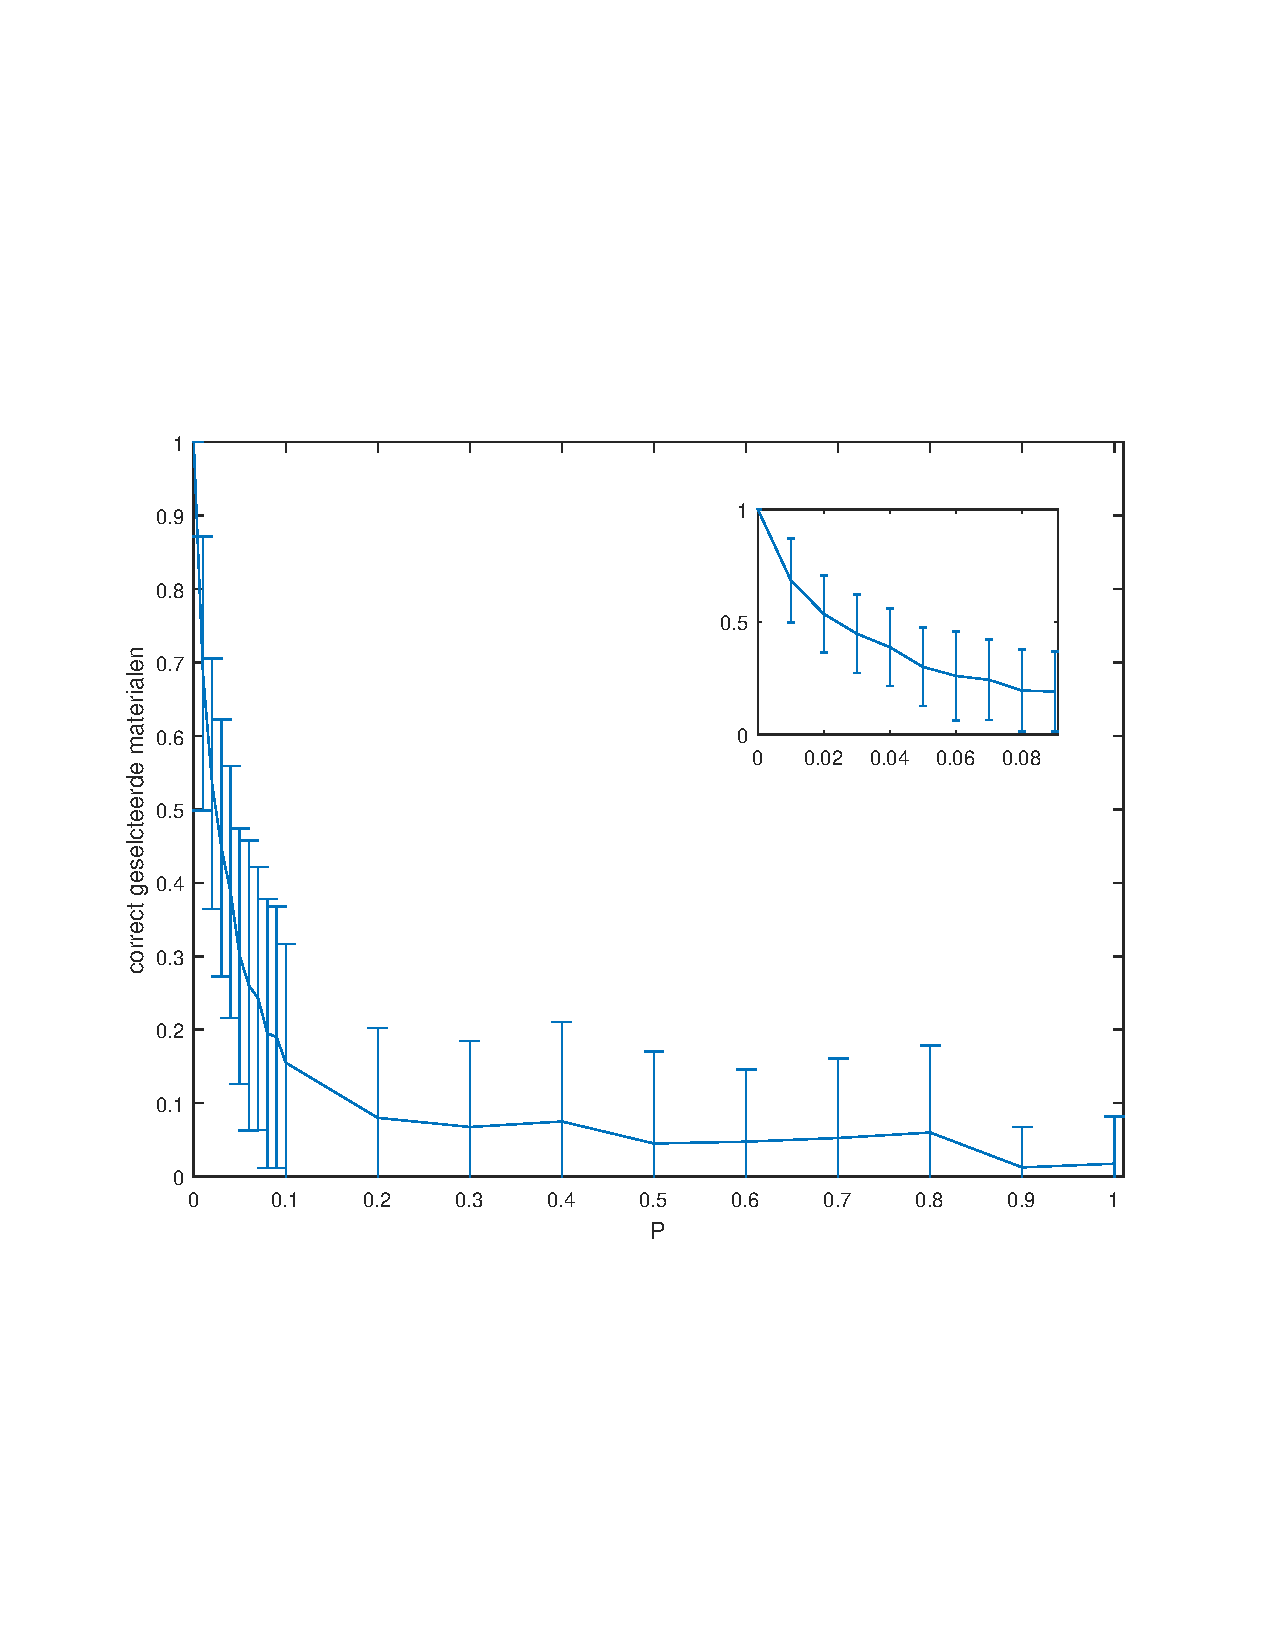
\includegraphics[width=0.49\linewidth,trim=0 200 0 175 cm]{export_PMC_10_100_corr.pdf}
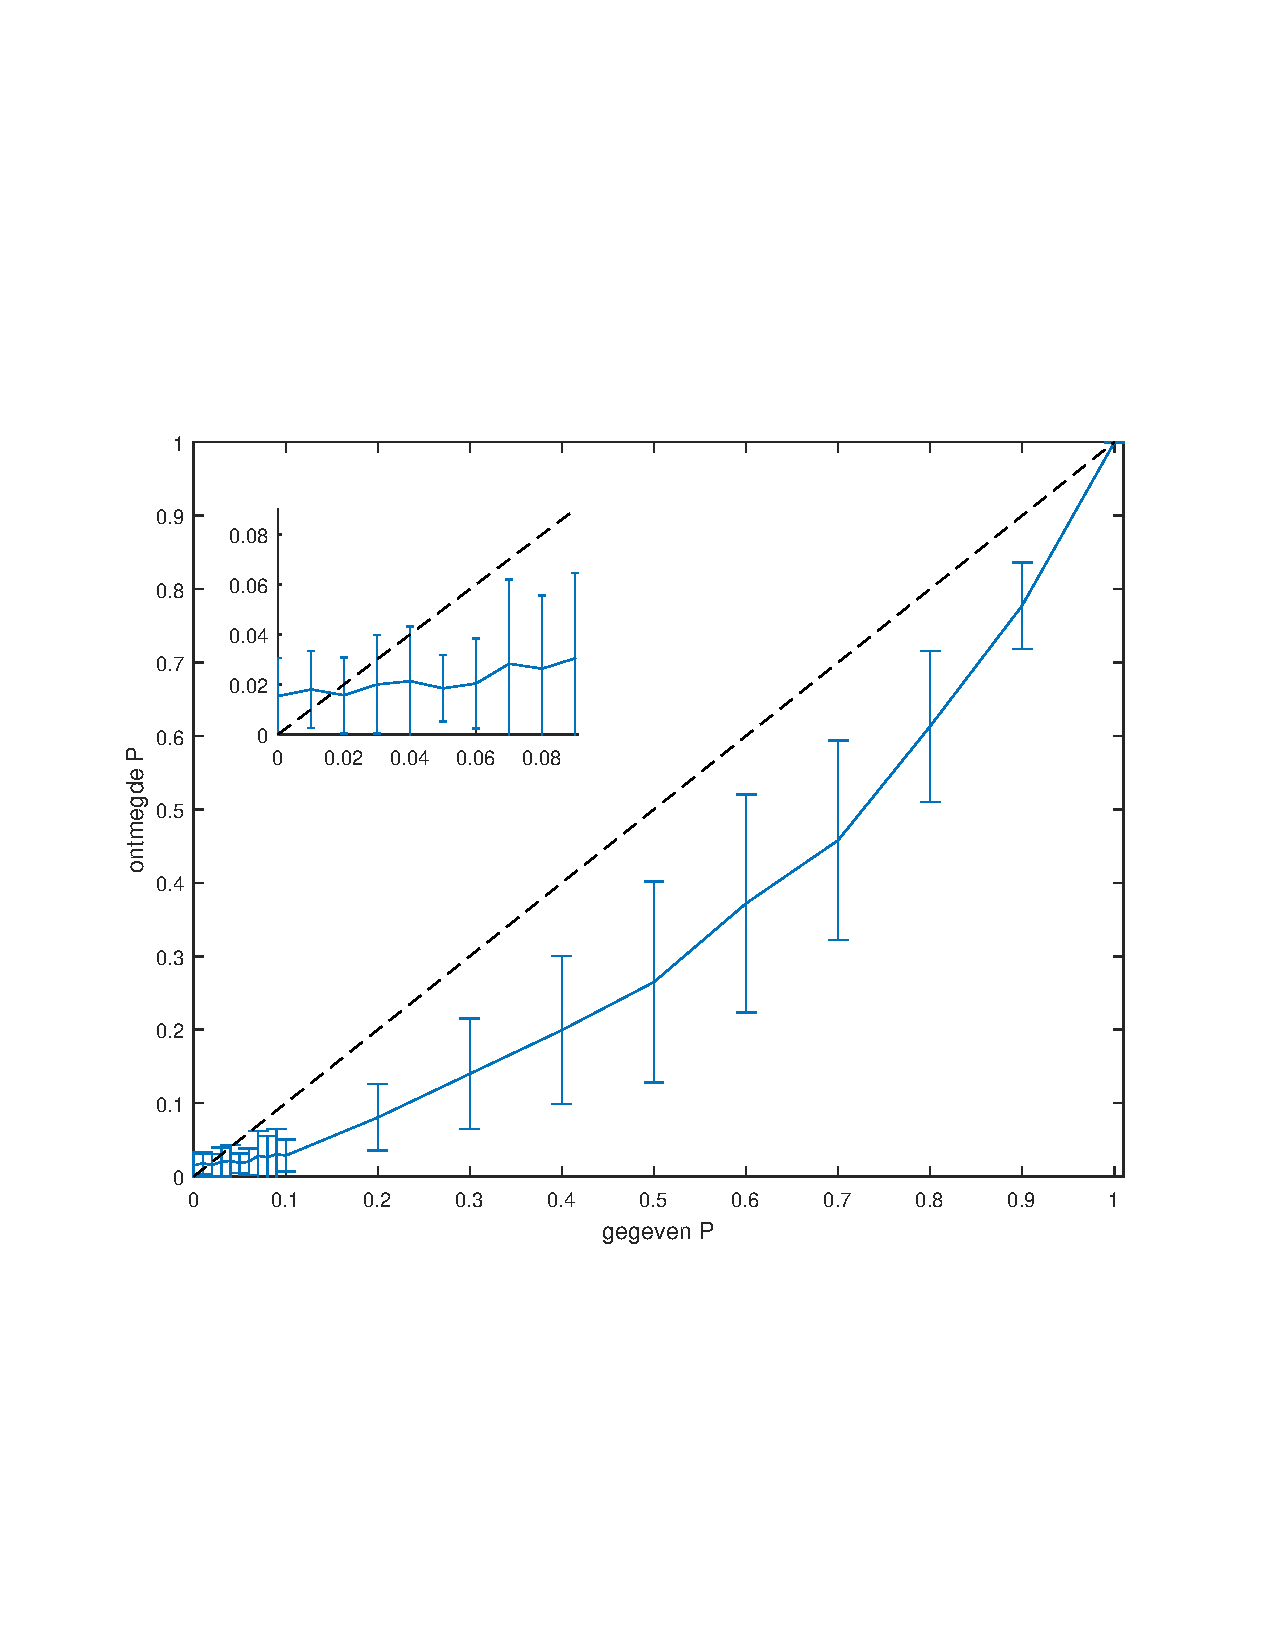
\includegraphics[width=0.49\linewidth,trim=0 200 0 175 cm]{export_PMC_10_100_PP.pdf}
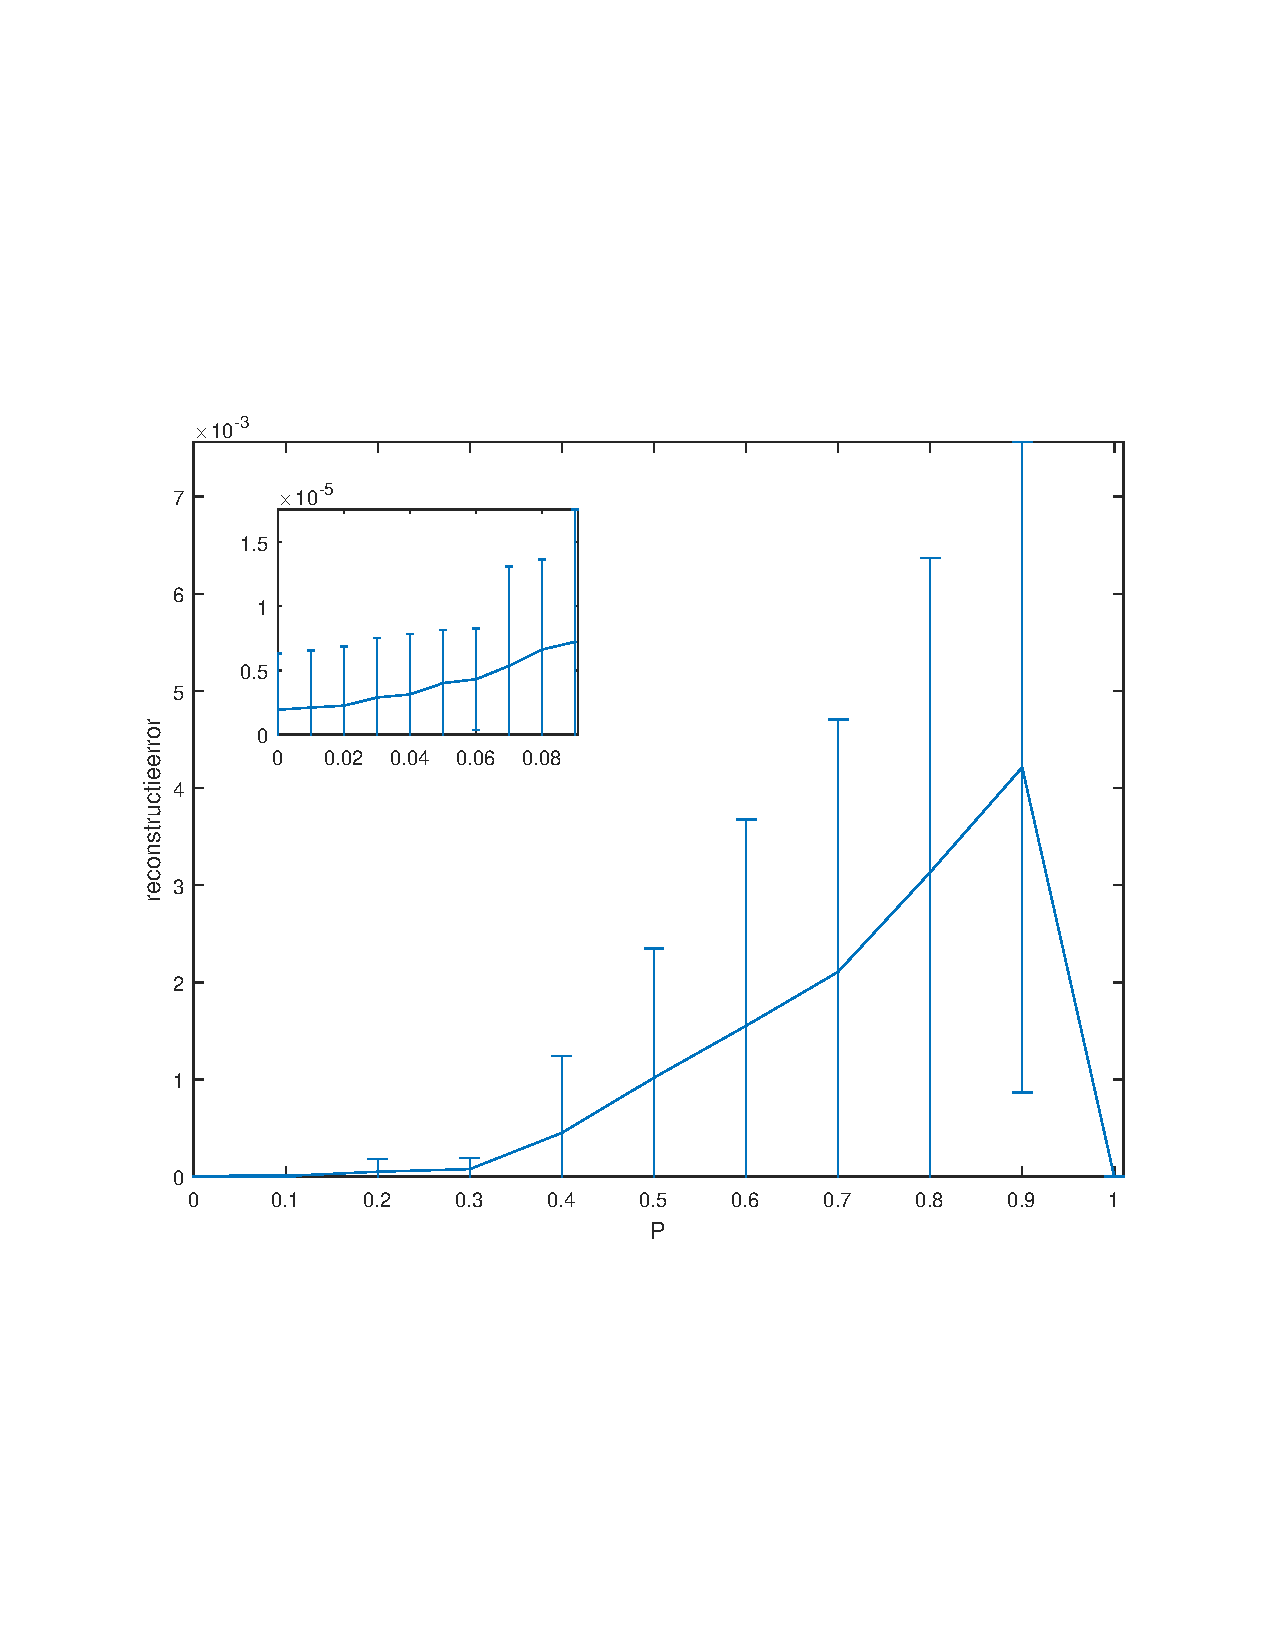
\includegraphics[width=0.49\linewidth,trim=0 200 0 175 cm]{export_PMC_10_100_E.pdf}
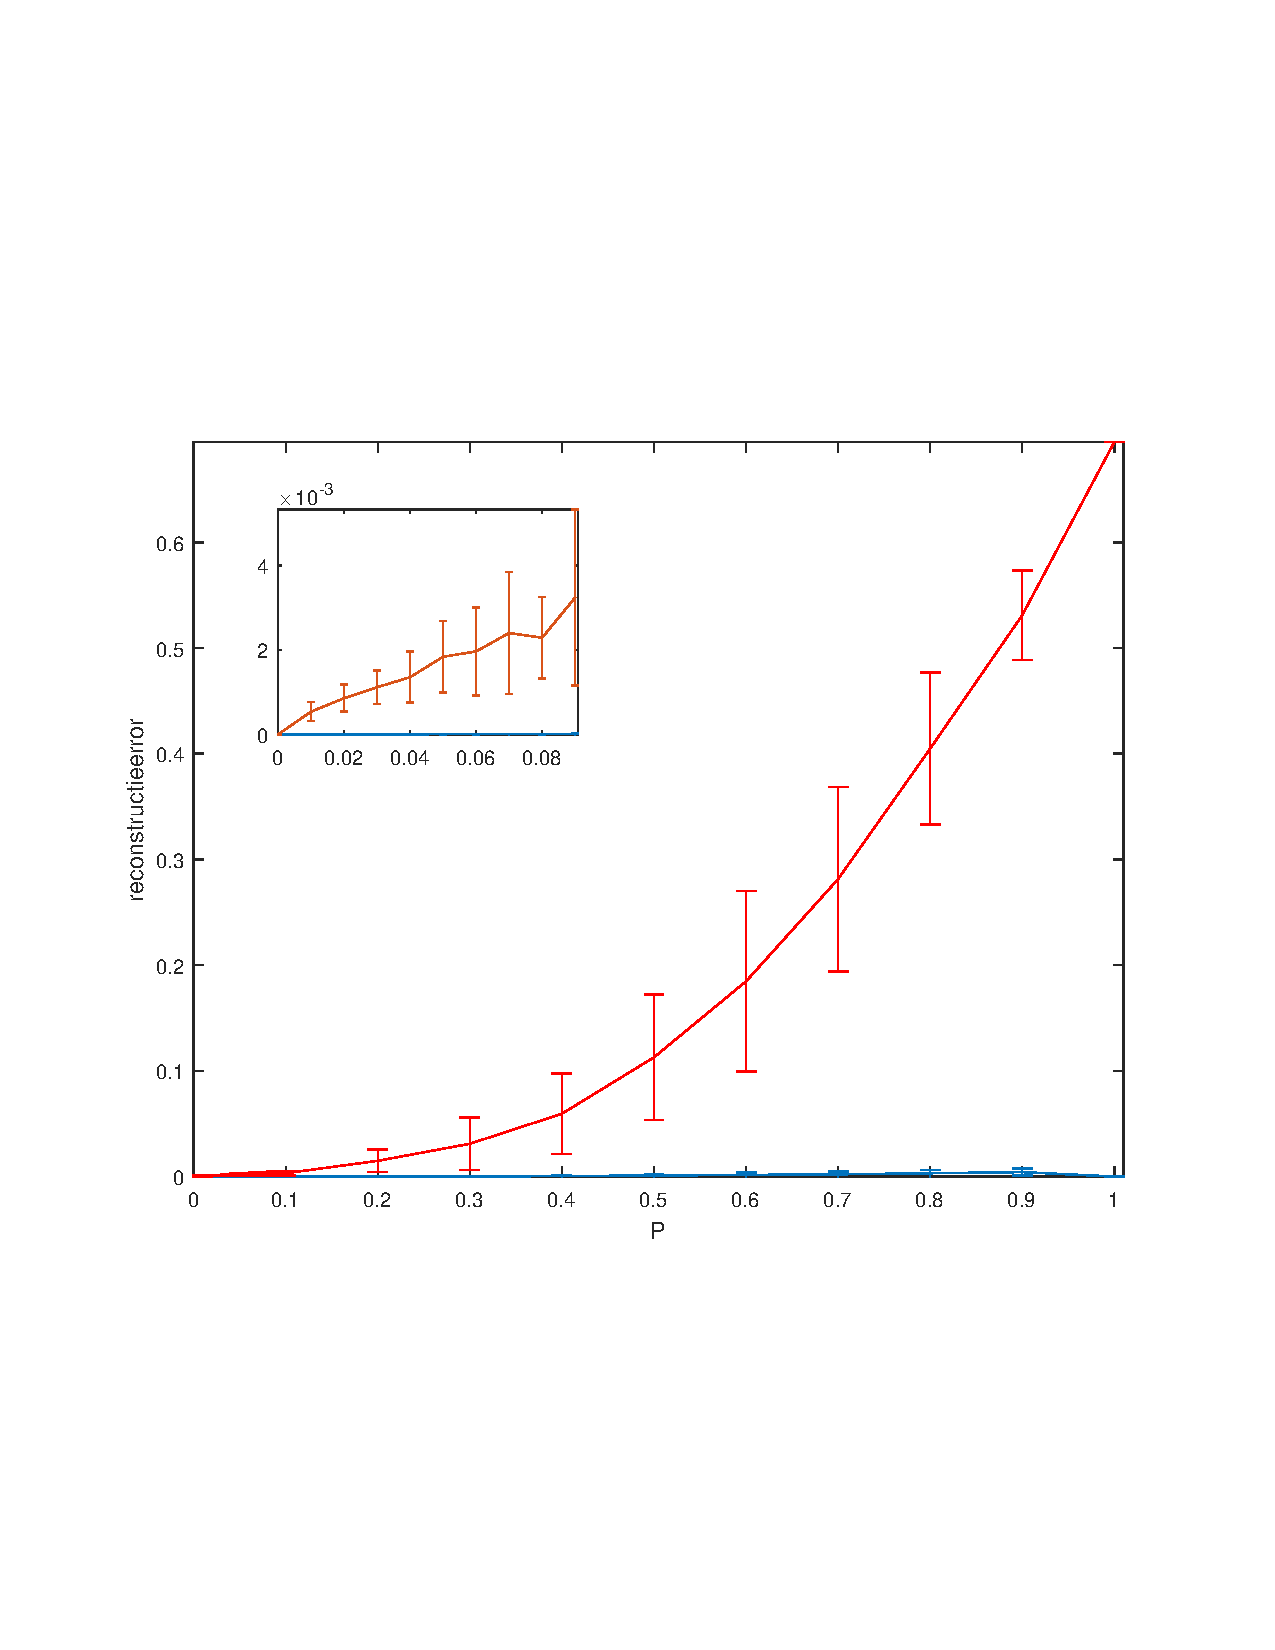
\includegraphics[width=0.49\linewidth,trim=0 200 0 175 cm]{export_PMC_10_100_El.pdf}
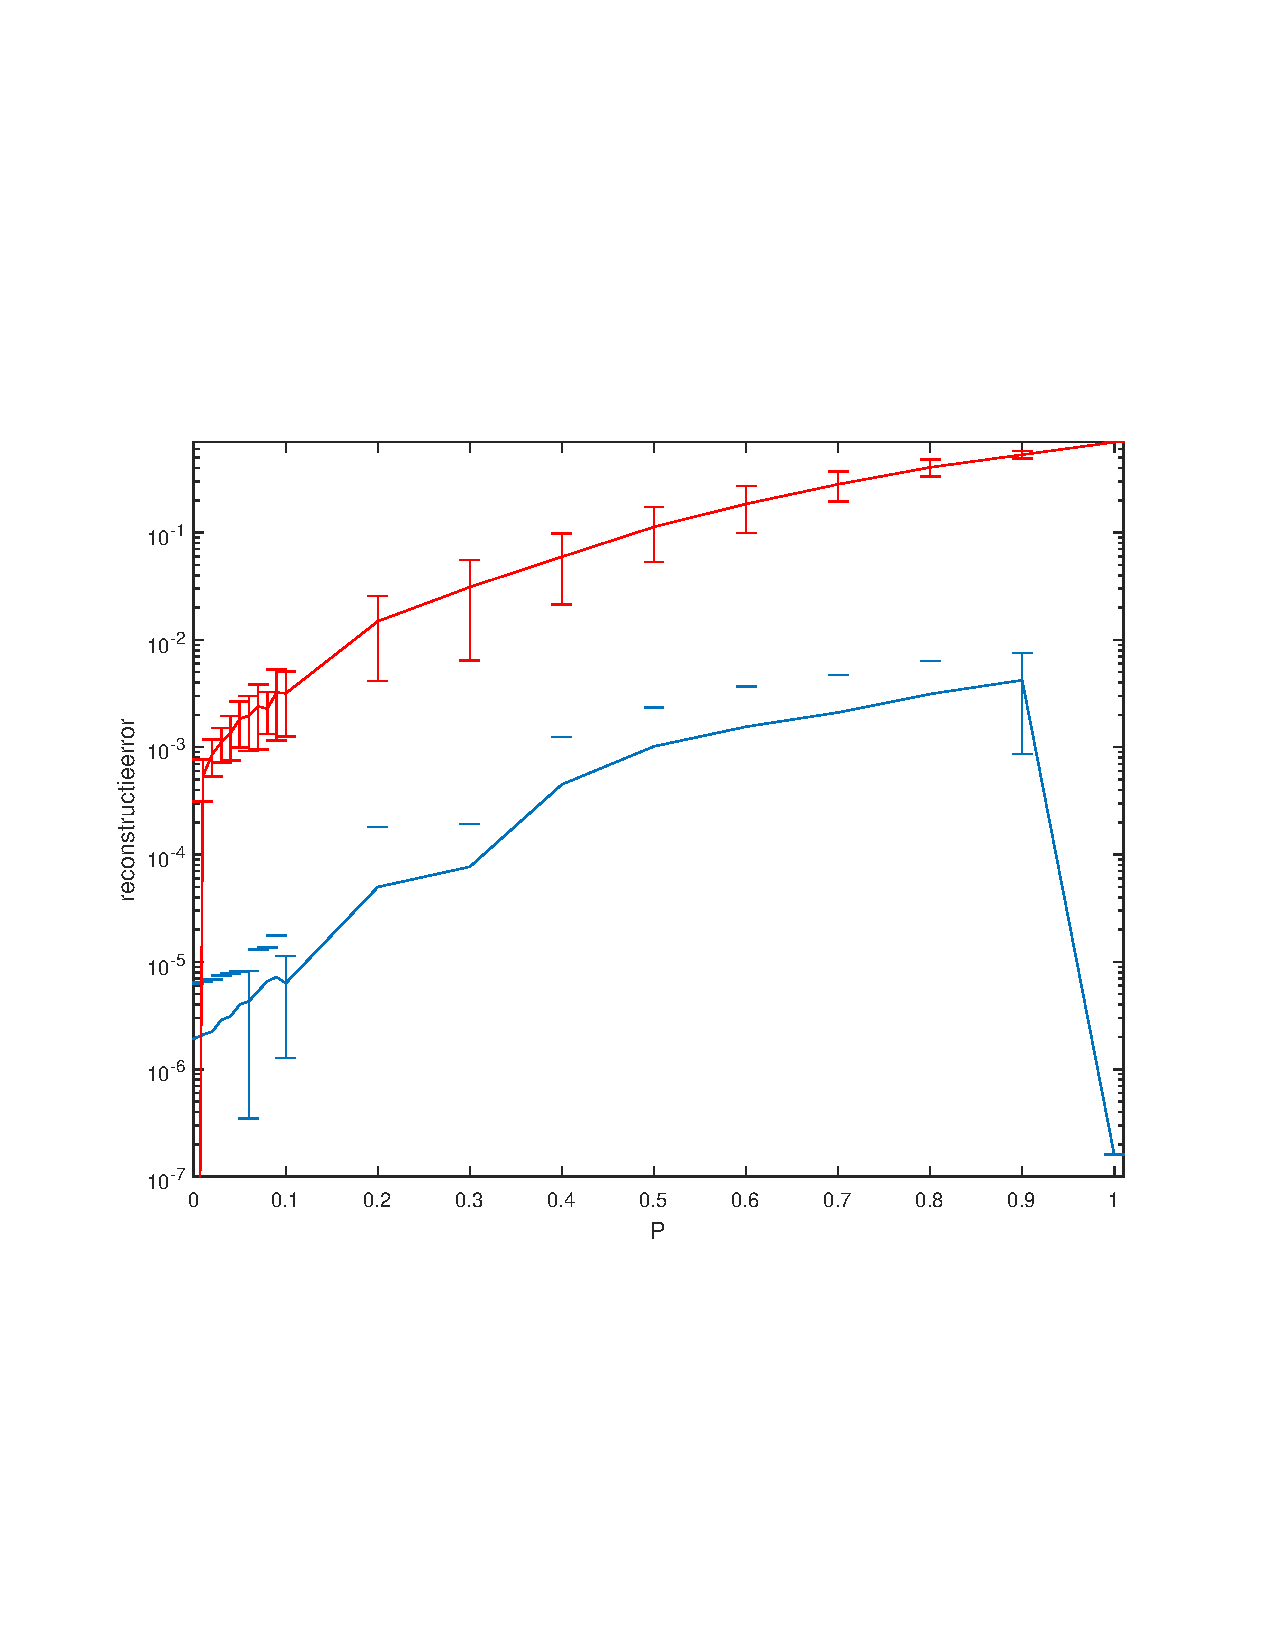
\includegraphics[width=0.49\linewidth,trim=0 200 0 175 cm]{export_PMC_10_100_Elog.pdf}
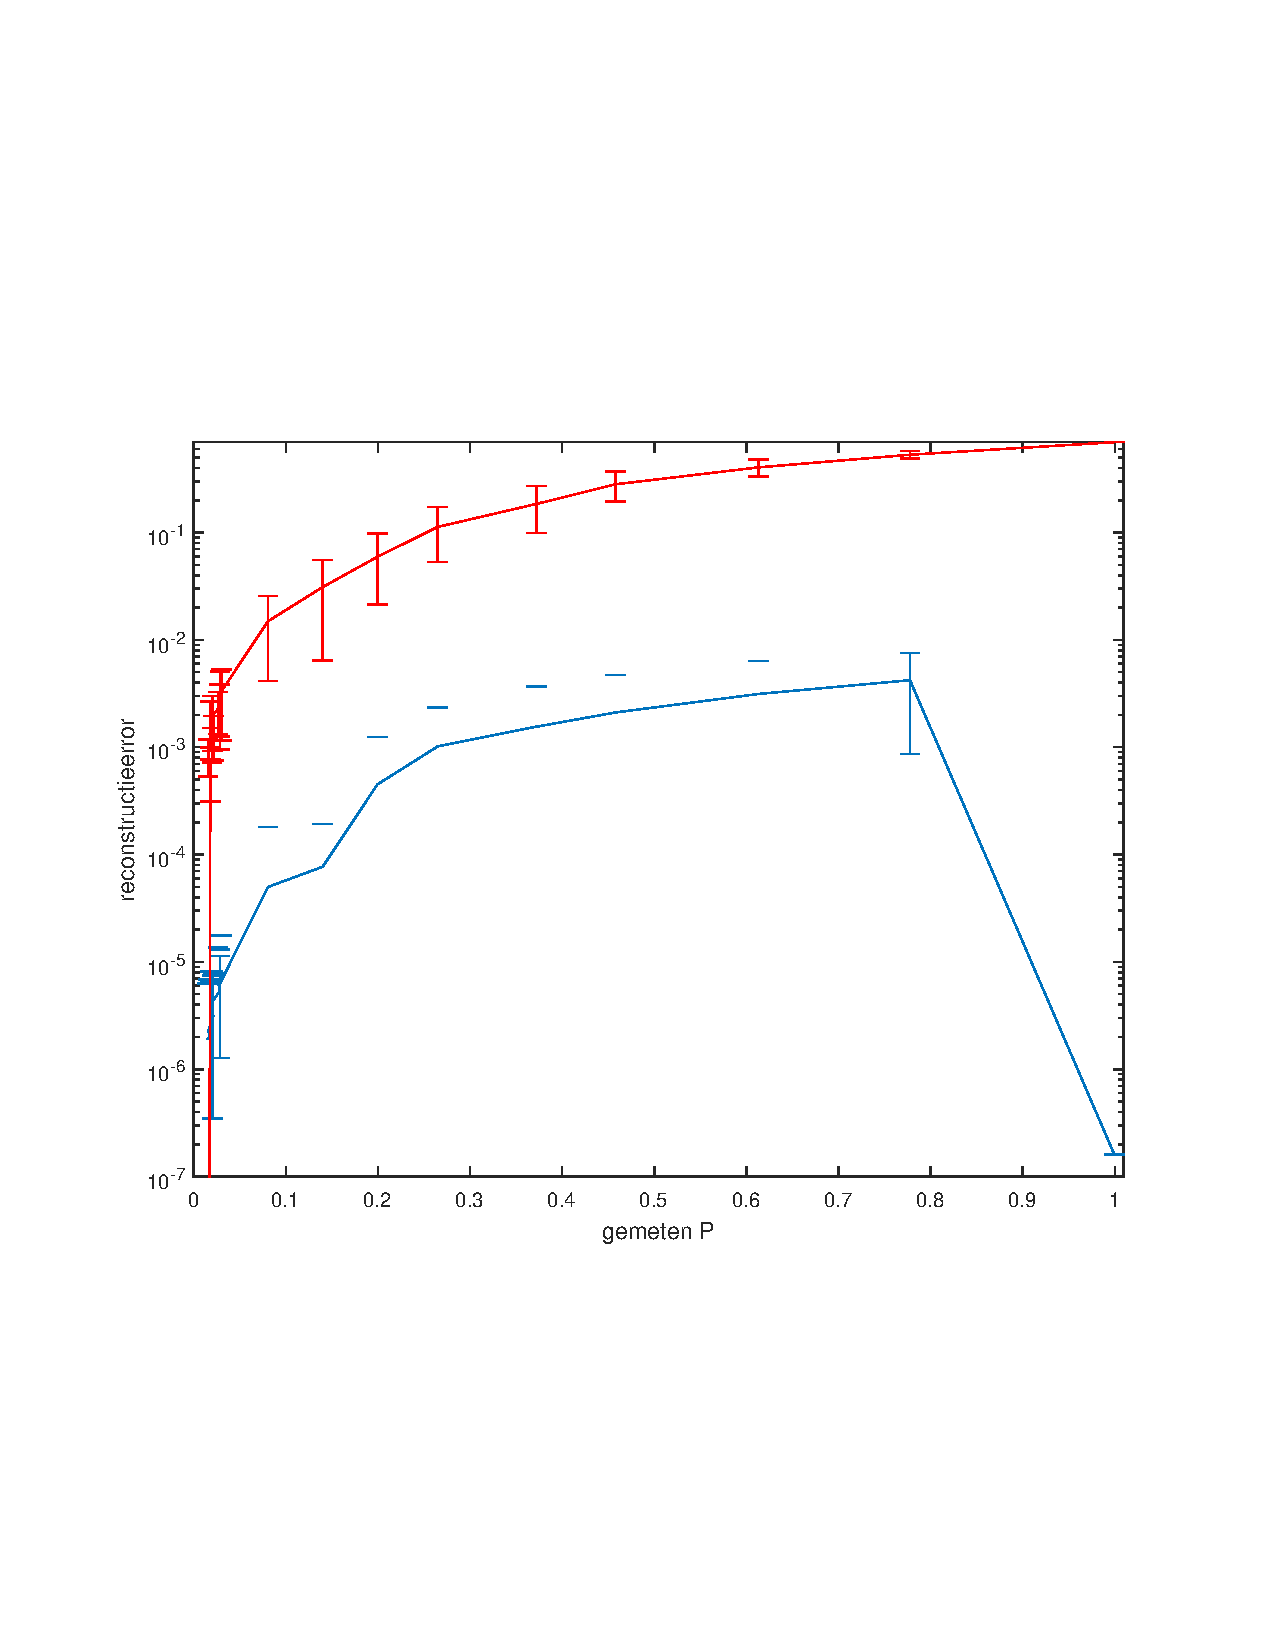
\includegraphics[width=0.49\linewidth,trim=0 200 0 175 cm]{export_PMC_10_100_EPlog.pdf}

\caption{Vergelijking tussen het lineair, semilineair en multilineair model. Voor elke $P$ waarde zijn er 100 pixels berekend. Rood is steeds het lineaire geval en blauw is het semilineair geval. Merkt trouwens op dat wanneer het eindpunt van de onderste foutenvlag onder nul ligt, alleen de bovengrens getekend is en niet de foutenvlag zelf op de logaritmische grafieken. Deze figuren zijn gemaakt met \textit{matlab}\cite{MATLAB}\label{fig:e100}}
\end{figure}

\begin{figure}
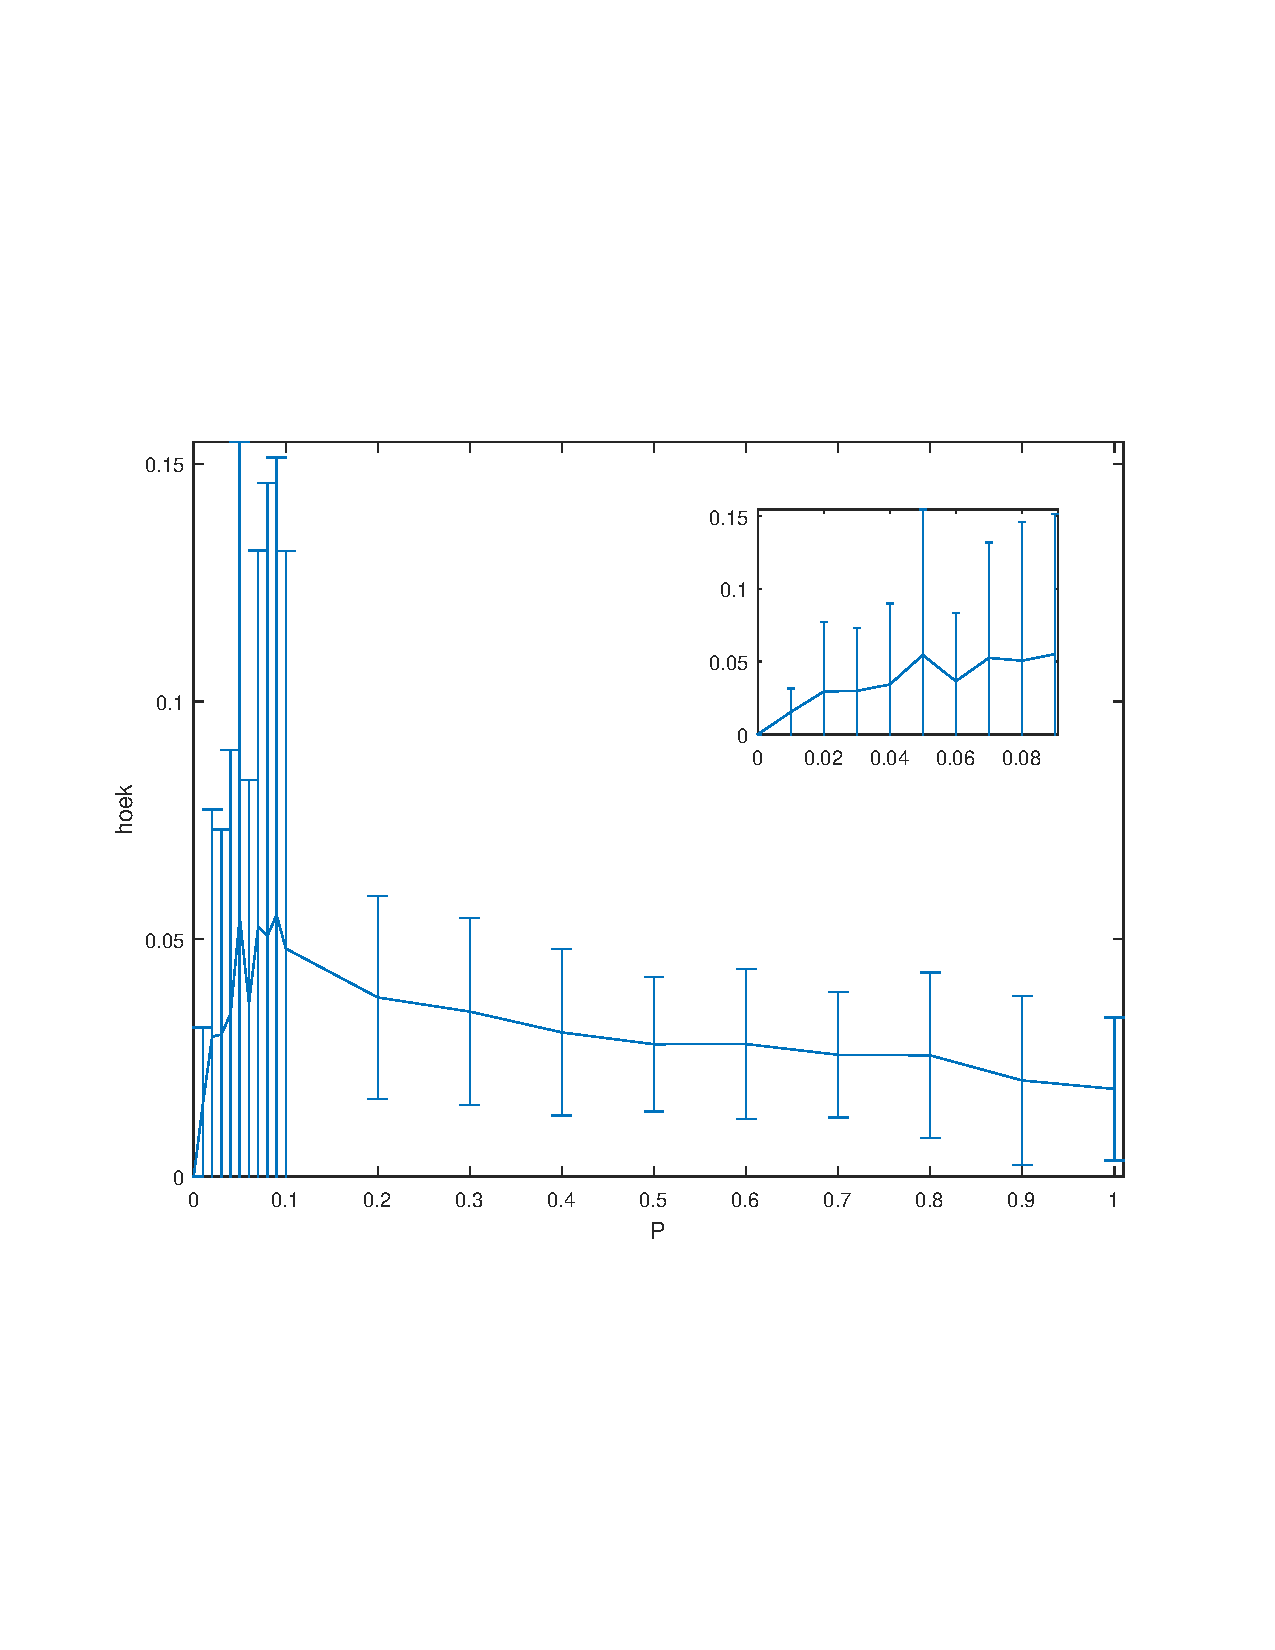
\includegraphics[width=0.49\linewidth,trim=0 200 0 175 cm]{export_PMC_10_100_angle.pdf}
\caption{Gevonden hoek in functie van de reflectie. Men ziet dat de foutenvlaggen veel groter zijn dan de data zelf.Deze figuren zijn gemaakt met \textit{matlab}\cite{MATLAB} \label{fig:hoek}}
\end{figure}

De verschillende data voor deze waarden kan gevonden worden in figuur \ref{fig:e100}. Het eerste wat kan opgemerkt worden is dat de standaardafwijking overal vrij groot is, en dat bijgevolg het resultaat sterk afhangt van de abundantie in de verschillende pixels. Als we kijken naar de reconstructie-error zien we dat deze relatief klein blijft voor lage $P$ waarden. Aangezien voor hogere waarden de benadering met de albedos gemaakt in vorige sectie toch niet meer geldt,  is dit geen probleem, aangezien beide modellen daar niet meer geldig zijn. In beide gevallen is de reconstructie-error ongeveer twee grootteordes kleiner dan die van het lineaire model. De rede dat de reconstructie-error keldert voor een waarde in de buurt van een, is omdat het mengingsalgoritme niet meer correct werkt voor deze waarden, en deze ook niet fysisch relevant is. Als de reflectie 1 is, zal een lichtstraal blijven reflecteren en nooit op de detector vallen.

Als we kijken naar de `correctheid' zien we dat de meeste materialen niet correct geselecteerd worden, aangezien dat de waarde voor $P=0.03$ al onder de helft ligt. Dit heeft weinig invloed op de reconstructie-error, aangezien het anders geselecteerde materiaal een goede benadering is voor het oorspronkelijke spectrum.

Kijken we naar de gemeten $P$ waarden dan zien we dat deze consequent lager zijn dan de gegeven $P$ waarden. Dit is wat verwacht wordt aangezien de elementen geselecteerd zijn met een algoritme dat lineair is, wat wil zeggen $P=0$. Daarom gaan `meer lineaire' ontmengingen sneller gekozen worden en wordt de interne reflectie dus lager. Dit is een probleem om bij een ontmengde waarde te bepalen hoe goed de reconstructie-error nog is aangezien deze afhankelijk is van $P$ en we de `echte' $P$ niet kunnen meten, alleen de `gemeten` $P$. Daarom staat er nog een extra grafiek, namelijk de reconstructie-error in functie van de gemeten $P$ in plaats van de echte $P$.

Om te weten te komen hoe goed de nieuwe bibliotheekelementen lijken op de oude, kan gebruik worden gemaakt van de hoek tussen deze twee spectra. Maar  zoals te zien in figuur \ref{fig:hoek} zijn de foutenvlaggen op deze waarden veel groter dan de waarden zelf, dus kan uit deze grafiek weinig afgeleid worden.

\subsubsection{maximale reflectie}

Op de grafieken is te zien dat de reconstructieerror van het semilenaire model exact nul wordt als $P=1$. Op zich is dit geen probleem aangezien deze situatie in werkelijkheid niet zal voorkomen en ook niet fysisch relevant is. Als een lichtstraal een kans van $1$ heeft om terug op het materiaal te vallen, zal deze nooit op de detector vallen. Uit vergelijking 35 volgt:

\begin{align}
\bm{x} = \frac{\sum_{i=1}^p (1-P_i) a_{i} \bm{w}_{i}}{1-\sum_{i=1}^p P_i a_{i} \bm{w}_{i}}
\end{align}

Vullen we $P \rightarrow 1$ in dan krijgt men

\begin{align}
\bm{x} = 0
\end{align}

Dit geldt zowel voor de het reconstructiespectrum als het gemengde spectrum, en de reconstructieerror is dus de norm van de nulvector, en deze is nul.

\subsection{Experimentele controle} \label{sec:exp}

In deze sectie worden de reconstructie-errors en waarden van werkelijke data uit de \textit{Alina dataset}\footcite{alina} bepaald, aan de hand van de verschillende modellen. Hierbij ontmengen we de derde rij van pixels. Dit zorgt ervoor dat er nog maar 19 pixels ontmengd moeten worden in plaats van het volledige aantal pixels uit de dataset, wat dit haalbaar maakt voor het multilineaire algoritme te gebruiken. De x-as op de grafieken verderop die positie-gelabeld is komt overeen met de positie van de waarden op de x-as.

In figuur \ref{fig:runtime} is de looptijd van verschillende pixels weergegeven. Hierop is eenvoudig te zien dat het semilineaire model en het lineaire model ongeveer dezelfde looptijd hebben. Dit is echter voor een kleine dataset, merk op dat voor een groter aantal pixels het semilineaire model slechter schaalt dan het lineaire model, en voor een grotere bibliotheek ze allebei gelijkmatig schalen. De bottleneck zal in werkelijkheid altijd zitten in de bibliotheken en niet in de werkelijke ontmenging. In het multilineaire model zijn deze twee niet meer gescheiden en zien we dus een enorme toename in looptijd.

In figuur \ref{fig:errorsR} zijn de reconstructie-errors weergegeven. Merk op dat per definitie de reconstructie-error van het lineaire model groter is dan deze van het semilineaire model en deze van het multilineaire model, op numerieke berekeningserrors na. Ook is de reconstructie-error van de afhankelijke kansen per definitie kleiner dan deze van de onafhankelijke parameters. Maar zoals te zien op figuur \ref{fig:errorsR} is deze vermindering enorm klein. Aangezien dit een verdubbeling van de vrije parameters inhoudt, is dit geen verbetering op het model. Anderzijds is te zien dat voor sommige pixels het semilinaire model een enorme verbetering is op het lineaire model, en soms dat beide modellen equivalent zijn. Aan de andere kant hebben het semilineaire en het multilineaire model bijna altijd een weinig verschillende reconstructie-error. 

Ter conclusie is het semilineaire model een sterke verbetering in looptijd ten opzichte van het multilineaire model, met een zeer klein kwaliteitsverlies, terwijl dit ten opzichte van het lineaire model een sterke kwaliteitswinst is voor sommige pixels zonder te verliezen aan snelheid.

In figuur \ref{fig:q} is enerzijds het quoti\"ent van de lineaire en semilineaire reconstructie-error weergegeven en rechts de $P$ waarde berekend aan de hand van het semilineaire model. Men ziet dat de pixels waar het semilineaire algoritme een sterke verbetering geeft qua reconstructie-error, ook een hogere $P$ waarde hebben. Dit is logisch, aangezien het lineaire algoritme ervan uitgaat dat $P=0$. Merk ook op dat dit overeenkomt met de ground-truth voor eikenbomen. Aangezien eikenbomen een fractalischer oppervlak hebben dan bijvoorbeeld asfalt, wat meer naar rechts in de afbeelding ligt, verwachten we hier ook een hogere $P$ waarde. Ter conclusie: het semilineaire model is vooral een verbetering ten opzichte van het lineaire model voor gebieden met meer fractalische oppervlakken, zoals vegetatie.


\begin{figure}
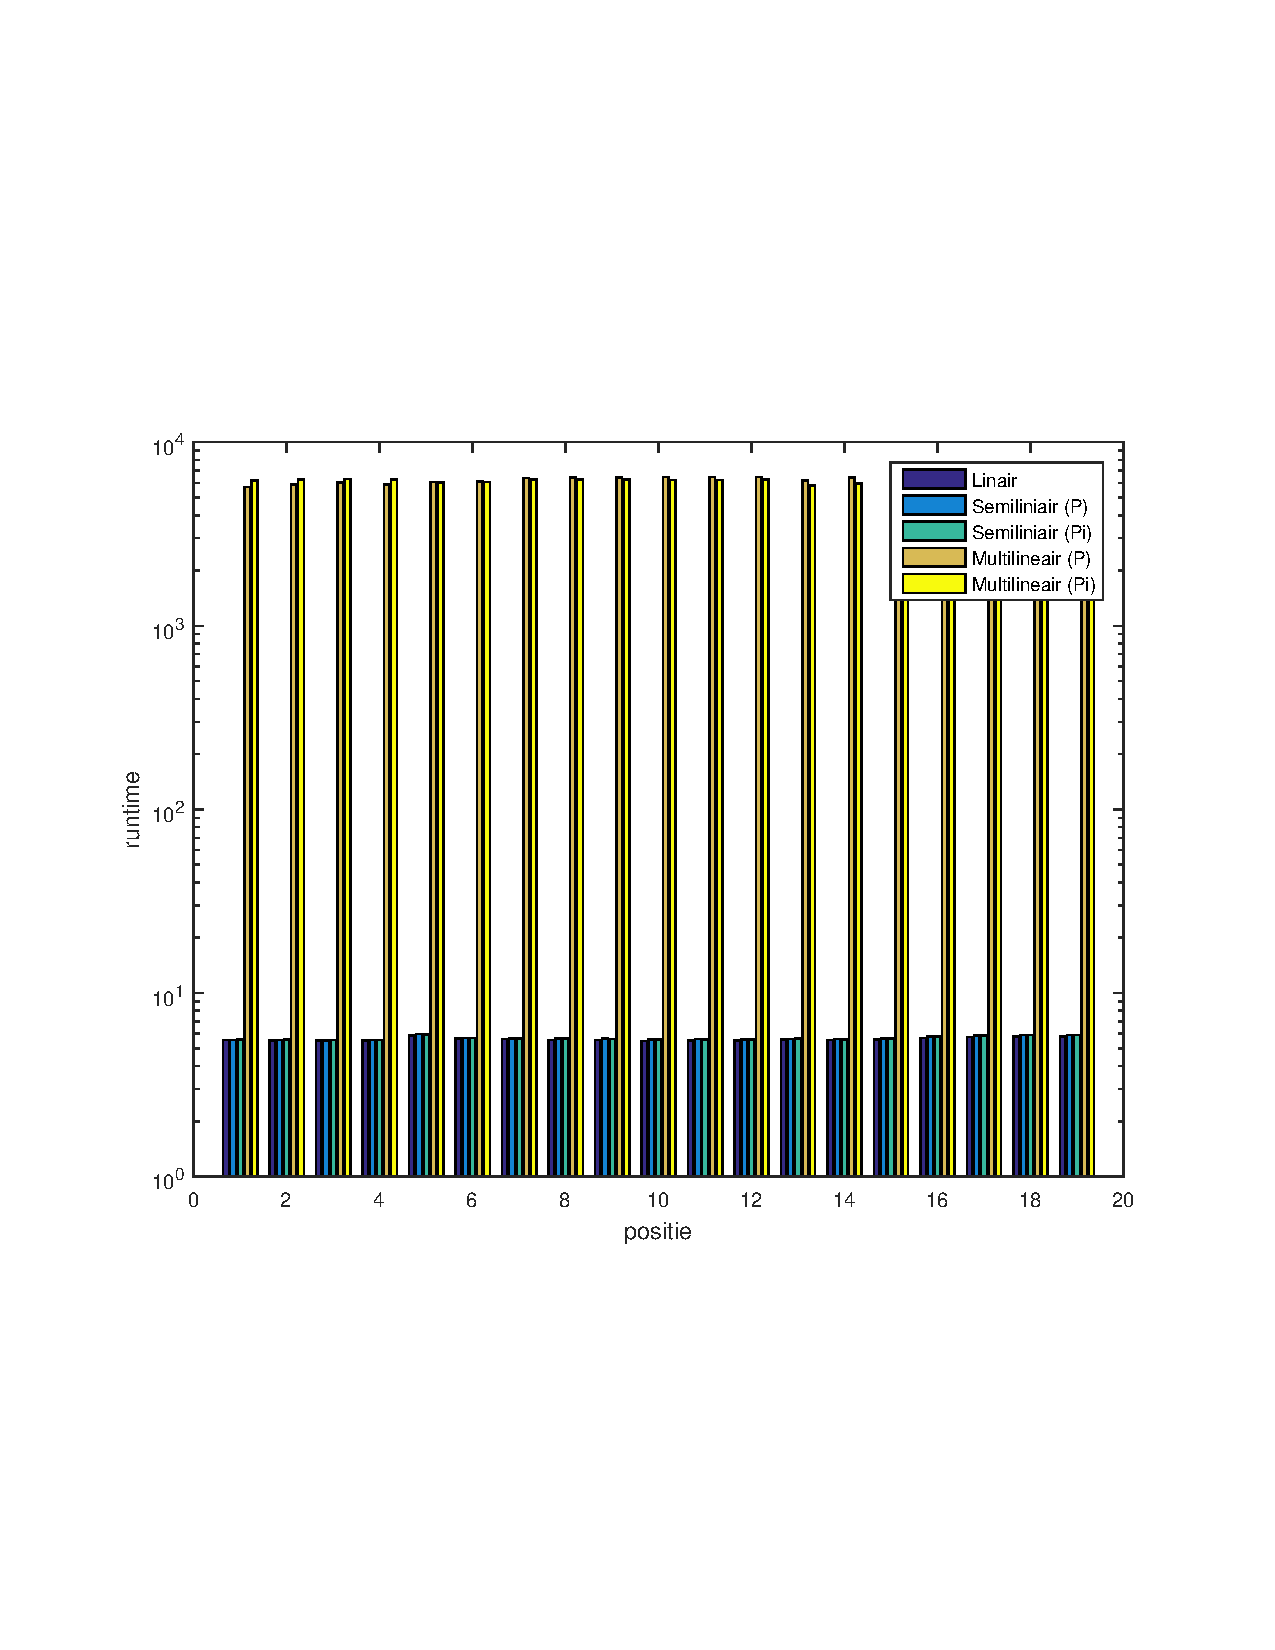
\includegraphics[width=0.79\linewidth,trim=0 200 0 175 cm]{exp_runtime.pdf}
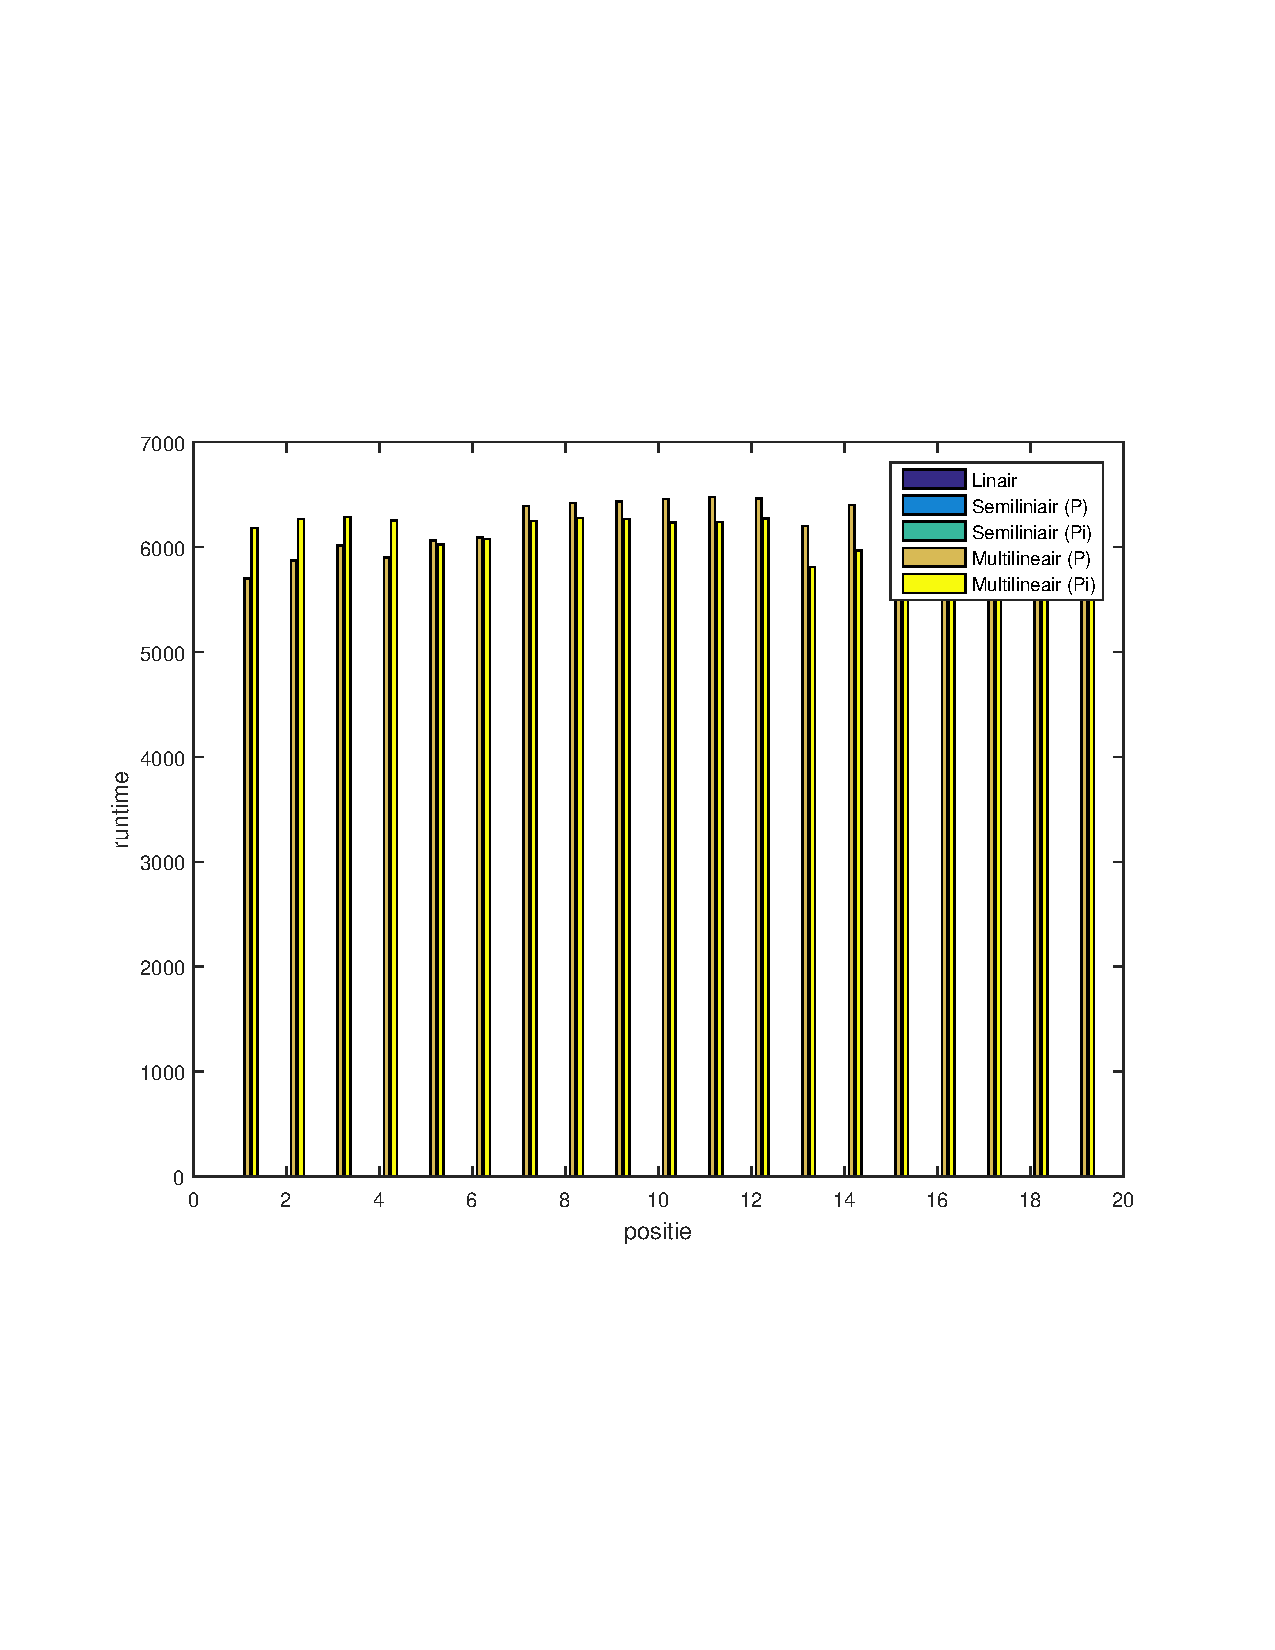
\includegraphics[width=0.79\linewidth,trim=0 200 0 175 cm]{exp_runtime_honest.pdf}
\caption{Looptijd van het programma voor de verschillende modellen. \texttt{(P)} betekent een onafhankelijke kans, \texttt{(Pi)} betekent een eindmember afhankelijke kans. Er is zowel een lineaire als logaritmische versie weergegeven. Deze figuren zijn gemaakt met \textit{matlab}\cite{MATLAB} \label{fig:runtime}}
\end{figure}

\begin{figure}
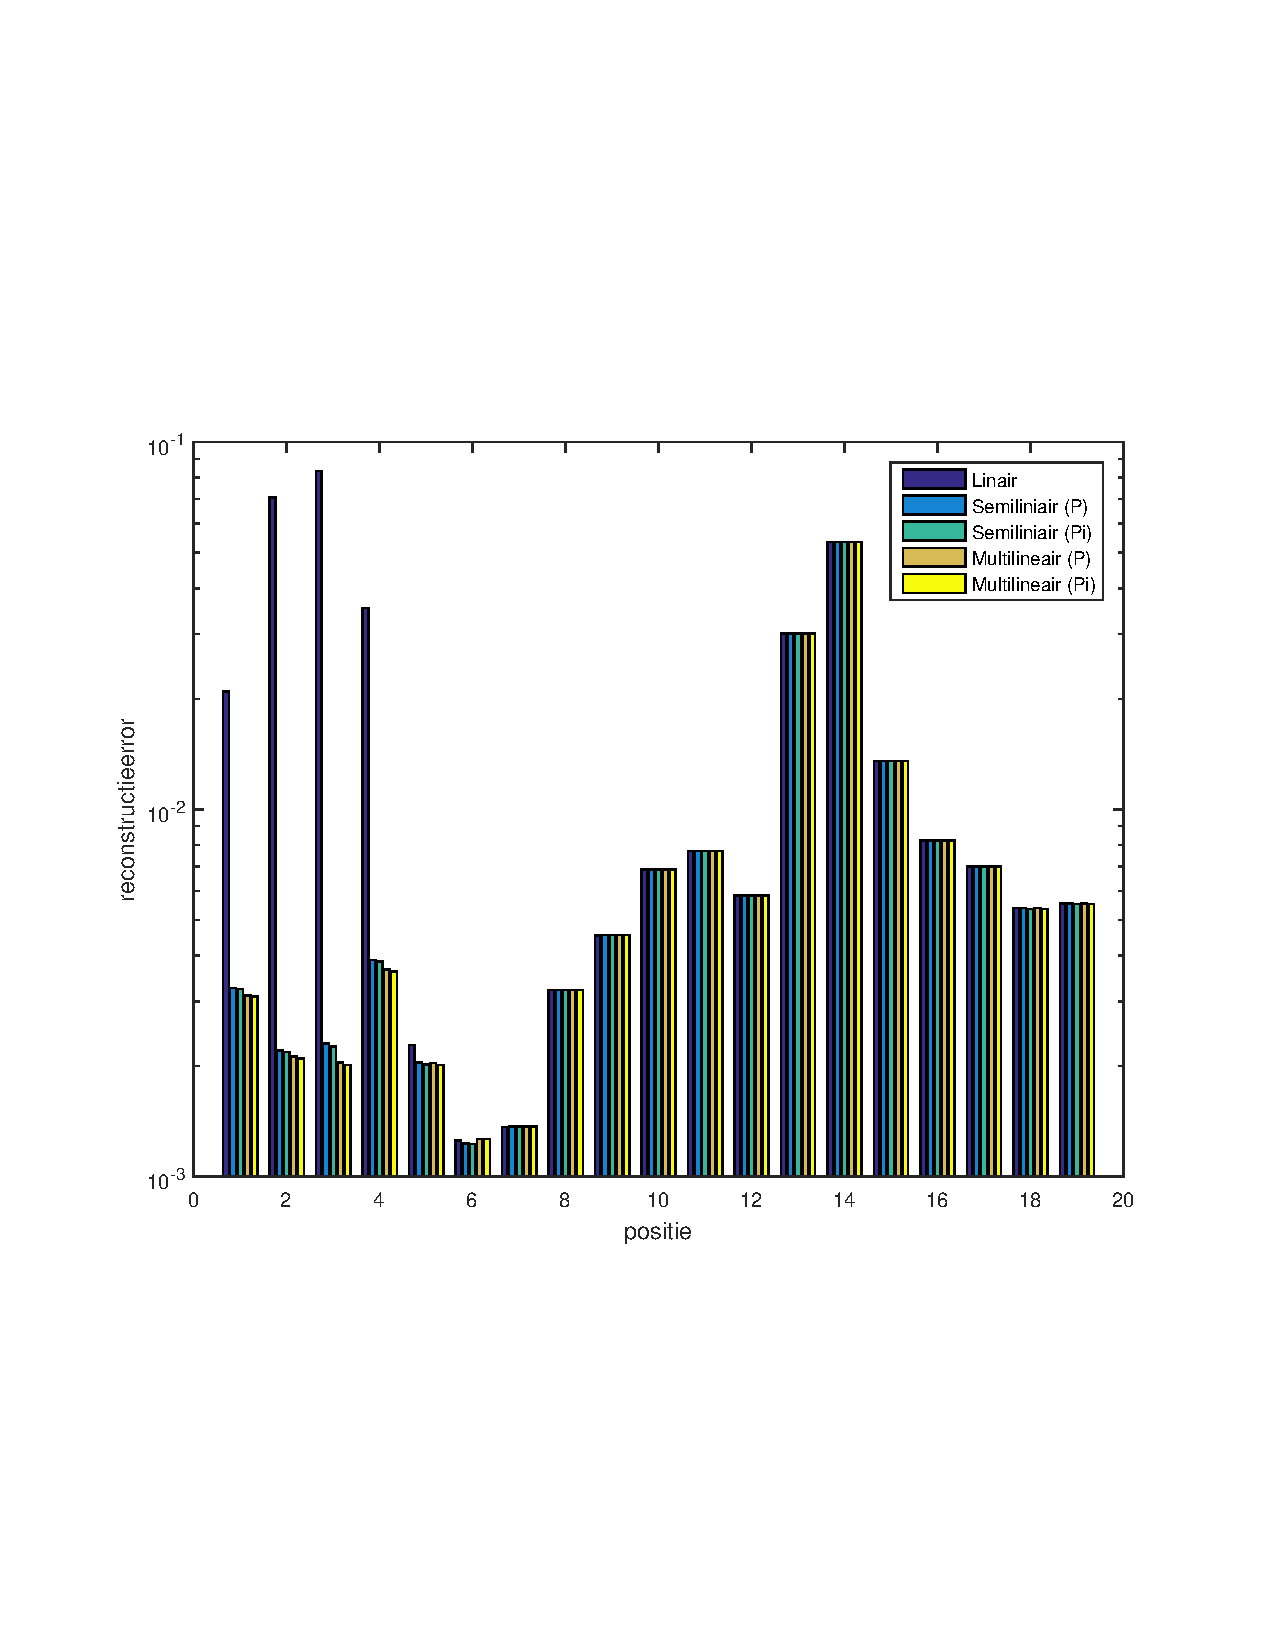
\includegraphics[width=0.79\linewidth,trim=0 200 0 175 cm]{exp_errors.pdf}
\caption{Reconstructie-error voor de verschillende modellen. \texttt{(P)} betekent een onafhankelijke kans, \texttt{(Pi)} betekent een eindmember afhankelijke kans. Deze figuren zijn gemaakt met \textit{matlab}\cite{MATLAB} \label{fig:errorsR}}
\end{figure}

\begin{figure}
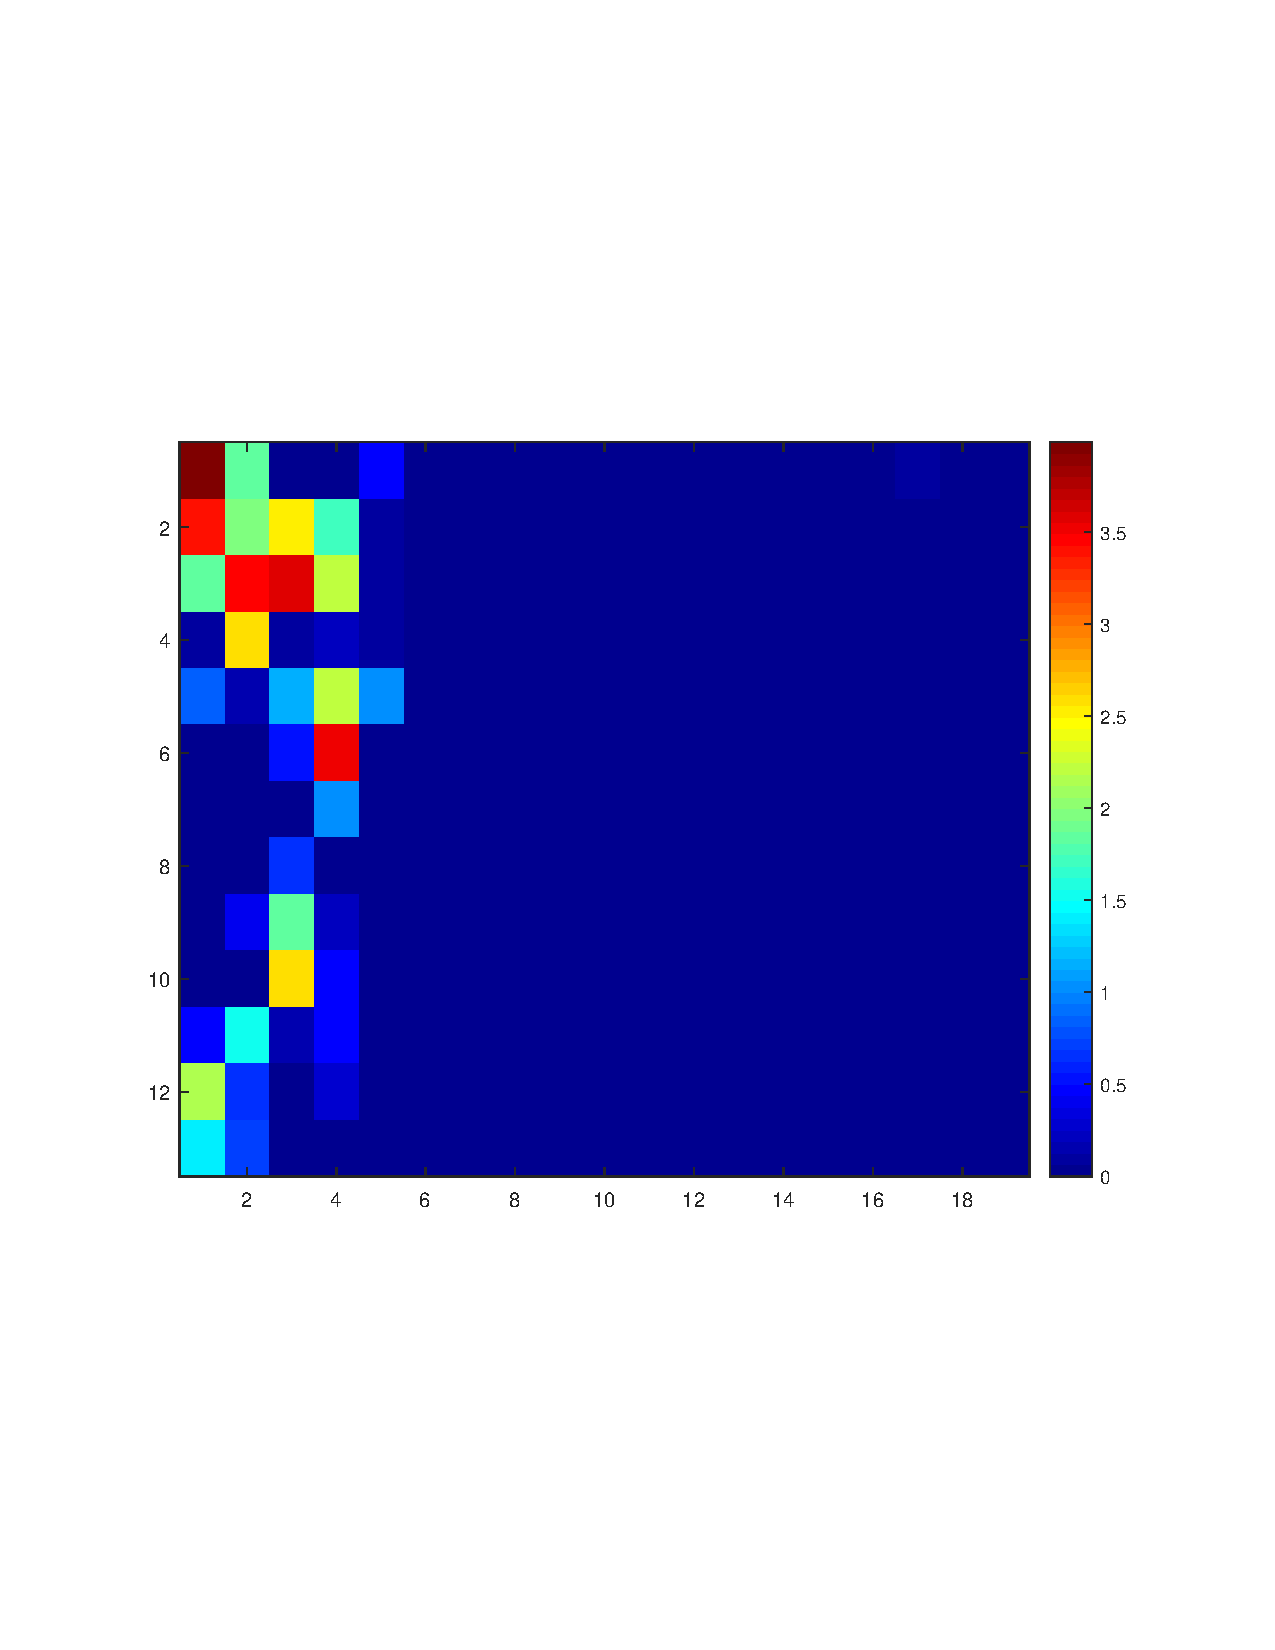
\includegraphics[width=0.49\linewidth,trim=0 200 0 175 cm]{Relative_Error.pdf}
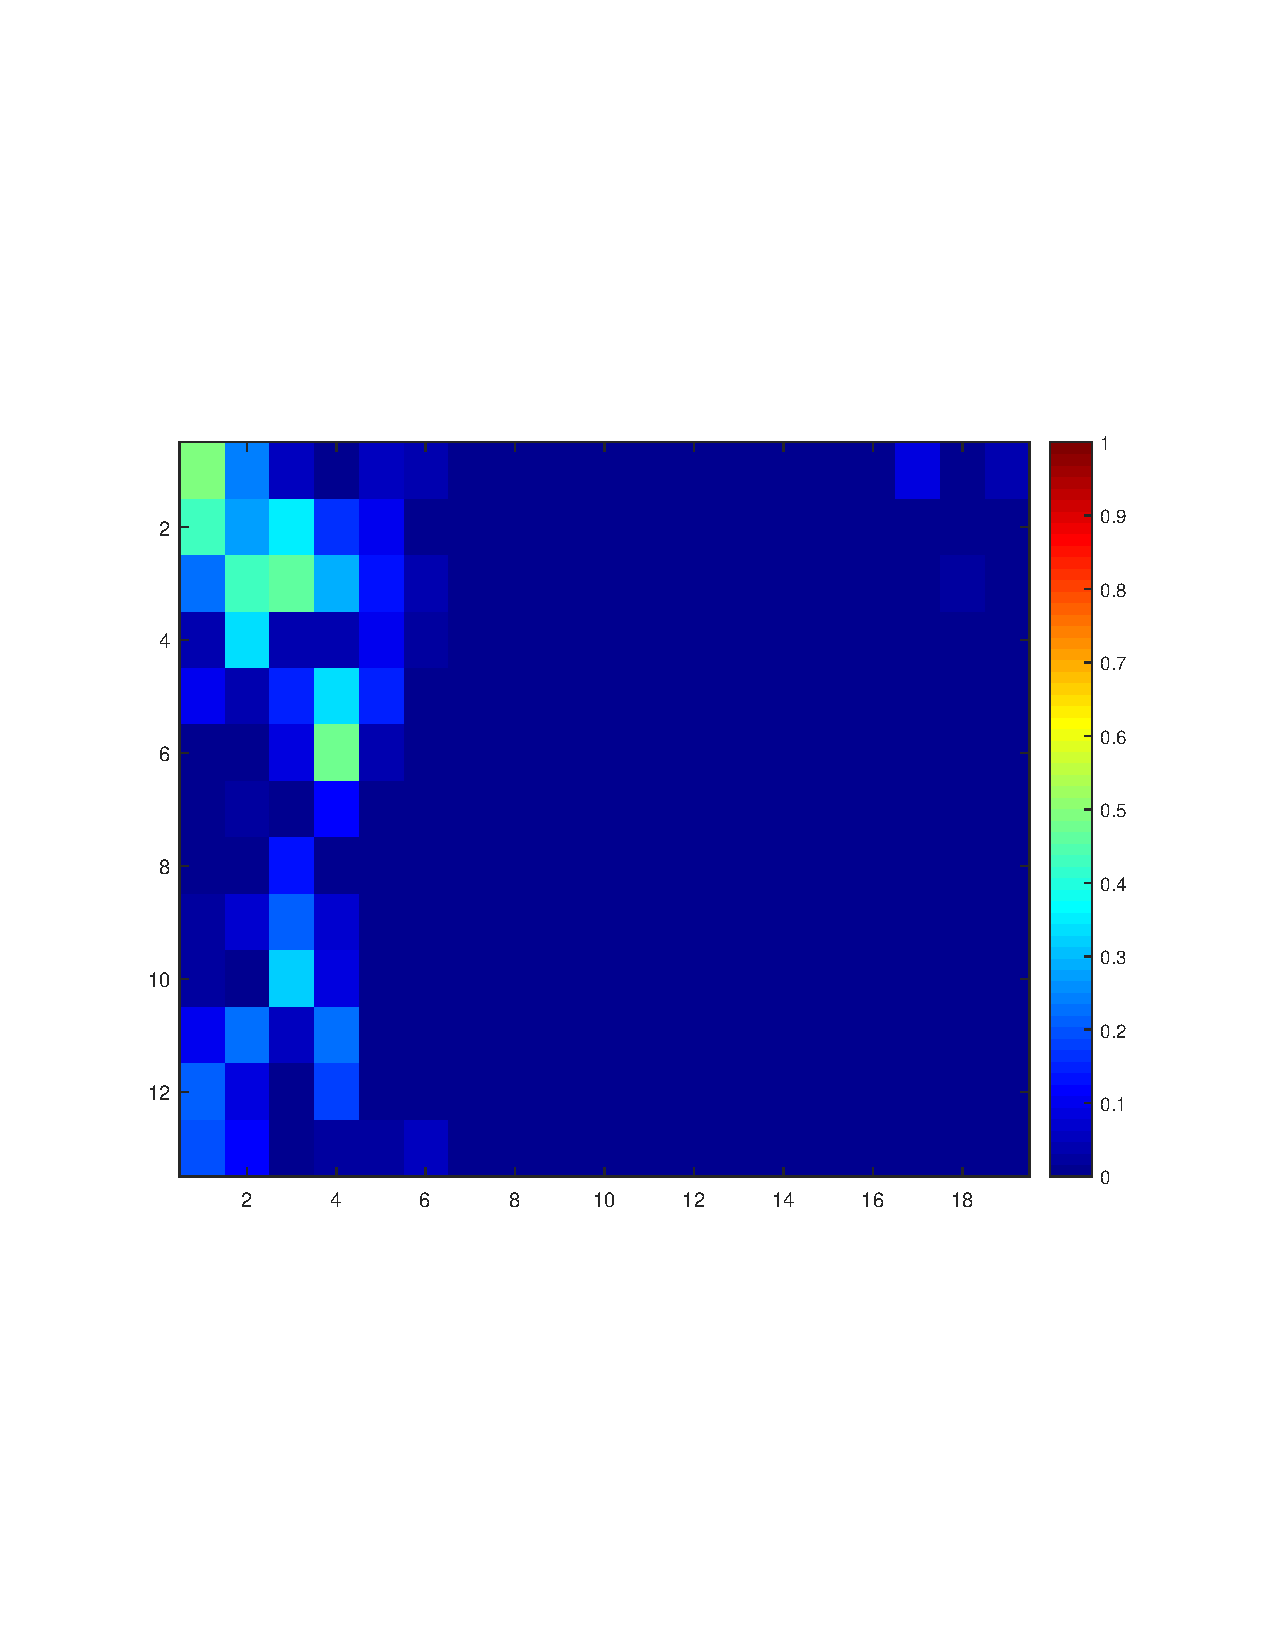
\includegraphics[width=0.49\linewidth,trim=0 200 0 175 cm]{P.pdf}
\caption{Relatieve reconstructie-error en reflexie voor de Alina dataset. Deze figuren zijn gemaakt met \textit{matlab}\cite{MATLAB} \label{fig:q}}
\end{figure}




%\section{Albedos meten}
%
%Van een willekeurig materiaal kan het reflectiespectrum gemeten worden. Uit vergelijking \ref{eq:Pi} volgt dat, wanneer er exact een materiaal aanwezig is:
%\begin{equation}
%\bm{w}_{i} = \frac{\bm{x}}{c_i\bm{x} + b_i}
%\end{equation}
%Aangezien als $a_i = 1$ geldt dat $c_i = P_i$ en $b_i = 1 - P_i$ geldt:
%\begin{equation}
%\bm{w}_{i} = \frac{\bm{x}}{P_i\bm{x} + 1 - P_i}
%\end{equation}
%Als $\bm{x}$ en $P_i$ bekend zijn, kan dit gewoon gemeten worden. In werkelijkheid kan $\bm{x}$ gewoon gemeten worden, maar is het bijna onmogelijk om $P_i$ te bepalen. We kunnen dit als extra parameter aan het systeem toevoegen.
%
%We hebben nu per materiaal 3 vrijheidsgraden, $b_i$,$c_i$ en $R_i$. Waarbij $R_i$ de reflectiekans is. Deze wordt verderop $R_i$ genoemd om verwarring te voorkomen met de $P_i$ in de pixel.Merk op dat $b_i$ en $c_i$ pixelafhankelijk zijn in tegenstelling tot $R_i$, welke dezelfde waarde heeft voor alle pixels.

%\subsection{berekening in matlab}
%
%In matlab worden de reflectiespectra en de albedo's voorgesteld als een matrix met elke rij het reflectriespectrum of albedo van een enkele endmember en de reflectiekansen als een vector. Dus geldt:
%
%\begin{equation}
%W_{ij} = \frac{X_{ij}}{\bm{P}_i X_{ij} + 1 - \bm{P}_i}
%\end{equation}
%
%Definieren we een matrix met dezelfde grootte als $X$ en waarbij elke colom overal dezelfde waarde $P_i$, dus $P_{ij} = P_i$ dan kan de bovenstaande formule ontbonden in een vergelijking voor elk matrixelement. Dus kunnen de elementgewijze operaties van matlab hier gebruikt worden.

%\subsection{pixelonafhankelijke waarden} %Nagel aan mijn doodskist
% Sommige parameters die bepaald kunnen worden zijn onafhankelijk van de pixel die op dat momemt berekend wordt. Bijvoorbeeld de refelctiekans van de endmembers $R_i$ voldoet hieraan. Dit heeft als gevolg dat alle vergelijkingen voor alle verschillende pixels gekoppeld zijn. Dit zorgt ervoor dat er niet meer pixel per pixel bereknd kan worden, maar alle pixels tegelijk berekend moeten worden, wat computationaal veel zwaarder is. 
% 
% Een alternatieve methode is in de eerste berekining verondestellen dat oneze pixelonafhankelijke waarden toch pixelafhankelijk zijn. Dan zijn alle pixels terug ontkoppelt worden de berekeningen terug eenvoudiger. Alleen blijft men dan over met een set mogelijke waarde voor deze variablen, terwijl deze maar \'e\'en echte waarde heeft. Daarom nemen we van al deze waarden de modus. Hoe de modus van een continue variable berekend kan worden staat bescheven in appendix \ref{sec:modus}. Nu ontstaat het probleem dat deze waarden gekoppeld zijn met de pixelafhankelijke waarden. Als een bepaalde pixel een uitschieter was, zouden de aandere waarden mee moeten aanpassen als een waarde veranderd wordt. Daarom wordt het algorimte om deze variablen te bepalen nog een keer gedraait, alleen wordt nu de pixelonafhenkelijke waarden constant verondersteld.



%\subsection{Meerdere monsters}
%
%Beschouw twee monsters van hetzelfde materiaal, die beide een verschillende reflectiekans hebben. Dit kunnen twee monsters zijn die een verschillende vorm hebben, of een verschillend oppervlak. Noem de verschillende reflectiekansen respectievelijk $R_i$ en $R'_i$. Zelfs als deze reflectiekansen onbekend zijn kan het albedo hier nog altijd uit ge\"extraheerd worden. %Of niet, aangezien dit ding niet convergeert :(
%
%\begin{align}
%\bm{w}_{i} &= \frac{\bm{x}}{R_i\bm{x} + 1 - R_i} \\
%\bm{w}_{i} &= \frac{\bm{x'}}{R'_i\bm{x'} + 1 - R'_i} \\
%\frac{\bm{x}}{R_i\bm{x} + 1 - R_i} &= \frac{\bm{x'}}{R'_i\bm{x'} + 1 - R'_i} \\
%\frac{R_i\bm{x} + 1 - R_i}{\bm{x}} &= \frac{R'_i\bm{x'} + 1 - R'_i}{\bm{x'}} \\
%\left(1 - \frac{1}{\bm{x}}\right)R_i - \frac{1}{\bm{x}} &= \left(1 - \frac{1}{\bm{x'}}\right)R'_i - \frac{1}{\bm{x'}} \label{eq:RR}
%\end{align}
%
%Definieer 
%\begin{align}
%\bm{\mathcal{Z}} &= 1 - \frac{1}{\bm{x}} \\
%\bm{\mathcal{Z}'} &= 1 - \frac{1}{\bm{x'}} \\
%\end{align}
%
%Nu is
%\begin{align}
% - \frac{1}{\bm{x}} +  \frac{1}{\bm{x'}} &= \mathcal{Z} - \mathcal{Z}'
%\end{align}
%
%en kan vergelijking \ref{eq:RR} herschreven worden als:
%
%\begin{align}
%\bm{\mathcal{Z}} R_i + \bm{\mathcal{Z}} &= \bm{\mathcal{Z'}} R'_i + \bm{\mathcal{Z'}} \\
%\bm{\mathcal{Z}} \left(R_i + 1\right) &= \bm{\mathcal{Z'}} \left(R'_i + 1\right)
%\end{align}





%\section{databanken}

%Een databank of bibliotheek bevat een aantal sets reflectiespectra, elk genomen in verschillende omstandigheden. Elk van deze set bevat de reflectiespectra van verschillende materialen. We proberen een bibliotheek te vinden dat het beste de omstandigheden beschrijft die aanwezig waren bij het nemen van het satelietbeeld. Hiervan selecteren we een deelverzameling van materialen die aanwezig zijn in het beeld en daarmee ontmengen we. Practisch zordt van elke mogelijke deelverzameling van elke set materialen het systeem ontmegt en daarmee het systeem eruit gehaald met de laagste error. Hierbij moet de voorkeur gegeven worden aan systemen met minder materialen, aangezien deze minder parameters moeten fitten en dus bijgevolg een hogere error hebben.

%Dit kan worden ingezien als volgt. Stel een systeem dat in werkelijkheid vier materialen bevat. Men kan bij de reconstructie een vijfde materiaal toevoegen %VERKEERD

%\subsection{selecteren van bibliotheken}

%\subsection{selecteren van endmembers}




%\section{gemiddelde error optimalisatie} %Dees werkt van geen kanten
%
%De correcte deelverzameling van de corrected bibliotheek wordt gekozen aan de hand van de laagste error, gemiddeld genomen over alle pixels. Dit betekend dat, aangezien de zelfde verzameling pixels gebruikt wordt voor elke bibliotheek, dat de bibliotheek met de laagste som van alle errors gebruikt zal worden. Dus als het algorimte bezig is met voor elke pixel de error te berekenen, en de totale error van de lokale pixels is groter dan de totale error van een van de vorige bibliotheken, dan is het niet nuttig om de error op de overige pixels te berekenen, aangezien de totale error automatisch groter  zal zijn dan deze vorige bibliotheek, en dus is deze bibliotheek zeker niet de correcte bibliotheek.


\chapter{vergelijking van verschillende ontmengingsmodelen}

\section{andere modellen}

\subsection{Hoekminimalisatie}

\subsection{Bilineair model}

%\subsection{Geoptimaliseerd multilineair algorimte}


\section{modeleigenschappen}

\subsubsection{parametervrijheid}

\begin{table}
\Large\center
\begin{tabular}{r|c c}
&$P>0$&$P>-1$ \\
\hline
afhankelijke $P$ & Real & Free \\
onafhankelijke $P$ & Strict & Strong
\end{tabular}
\caption{Benamingen van de verschillende parameteropties voor multilineair ontmengen}
\end{table}

\subsubsection{Iteratiesnelheid}

\subsubsection{Selectiemethode}

\subsubsection{Ontmengingsmethode}


\subsection{mogelijke verklaringen voor negatieve reflectiekans}

\subsubsection{naaste buur interactie}

\subsubsection{albedo vs reflectie}

\section{experimetele vergelijking van verschillende modellen}


\begin{table}
\centering
\begin{tabular}{|c|c|c|c|c|c|c|c|c|c|c|c|}
\hline
 &  &  &  &  &  &  &  &  &  &  &  \\
\hline
lineair (600) & 2.0173 & 83.5303 & 3.0000 & 0.8162 & 0.0000 & 0.0000 & 0.1838 & 0.0000 & 0.0000 & 0.0000 & 0.0000 \\
\hline
strict semilineair (600) & 2.0284 & 2.3042 & 4.0000 & 0.4928 & 0.0000 & 0.0000 & 0.5072 & 0.4538 & 0.0000 & 0.0000 & 0.4538 \\
\hline
real semilineair (600) & 2.0915 & 2.2637 & 7.0000 & 0.2836 & 0.0000 & 0.0000 & 0.7164 & 0.0078 & 0.0000 & 0.0000 & 0.6375 \\
\hline
strict AAM ML (600) & 0.0896 & 2.2376 & 4.0000 & 0.6209 & 0.0000 & 0.2153 & 0.1638 & 0.4716 & 0.0000 & 0.4716 & 0.4716 \\
\hline
strict AAM ML (60) & 0.0684 & 2.3583 & 4.0000 & 0.5339 & 0.0000 & 0.1338 & 0.3323 & 0.4750 & 0.0000 & 0.4750 & 0.4750 \\
\hline
strong semilineair (600) & 1.9924 & 2.3042 & 4.0000 & 0.4928 & 0.0000 & 0.0000 & 0.5072 & 0.4538 & 0.0000 & 0.0000 & 0.4538 \\
\hline
free semilineair (600) & 2.1435 & 2.2394 & 7.0000 & 0.1534 & 0.0000 & 0.0000 & 0.8466 & -0.8858 & 0.0000 & 0.0000 & 0.7061 \\
\hline
strong AAM ML (600) & 0.0863 & 2.2376 & 4.0000 & 0.6209 & 0.0000 & 0.2154 & 0.1637 & 0.4716 & 0.0000 & 0.4716 & 0.4716 \\
\hline
strong AAM ML (60) & 0.0681 & 2.2833 & 4.0000 & 0.5469 & 0.0000 & 0.1229 & 0.3301 & 0.4657 & 0.0000 & 0.4657 & 0.4657 \\
\hline
\end{tabular}
\caption{MyTableCaption}
\label{table:MyTableLabel}
\end{table}

\begin{table}
\centering
\begin{tabular}{|c|c|c|c|c|c|c|c|c|c|c|c|}
\hline
 &  &  &  &  &  &  &  &  &  &  &  \\
\hline
lineair (600) & 2.0019 & 6.9800 & 3.0000 & 0.3620 & 0.1524 & 0.4856 & 0.0000 & 0.0000 & 0.0000 & 0.0000 & 0.0000 \\
\hline
strict semilineair (600) & 2.0475 & 6.9809 & 4.0000 & 0.3612 & 0.1529 & 0.4859 & 0.0000 & 0.0013 & 0.0013 & 0.0013 & 0.0000 \\
\hline
real semilineair (600) & 2.0856 & 6.9795 & 7.0000 & 0.3543 & 0.1551 & 0.4907 & 0.0000 & 0.0004 & 0.0019 & 0.0165 & 0.0000 \\
\hline
strict AAM ML (600) & 0.0911 & 6.9809 & 4.0000 & 0.3612 & 0.1529 & 0.4859 & 0.0000 & 0.0013 & 0.0013 & 0.0013 & 0.0000 \\
\hline
strict AAM ML (60) & 0.0680 & 8.4695 & 4.0000 & 0.1729 & 0.2774 & 0.5497 & 0.0000 & 0.2399 & 0.2399 & 0.2399 & 0.0000 \\
\hline
strong semilineair (600) & 2.0374 & 6.9746 & 4.0000 & 0.3721 & 0.1459 & 0.4820 & 0.0000 & -0.0152 & -0.0152 & -0.0152 & 0.0000 \\
\hline
free semilineair (600) & 2.1099 & 6.5928 & 7.0000 & 0.2123 & 0.1368 & 0.6510 & 0.0000 & -0.8221 & -0.1494 & 0.3464 & 0.0000 \\
\hline
strong AAM ML (600) & 0.0902 & 6.9746 & 4.0000 & 0.3721 & 0.1459 & 0.4820 & 0.0000 & -0.0152 & -0.0152 & -0.0152 & 0.0000 \\
\hline
strong AAM ML (60) & 0.0681 & 7.0051 & 4.0000 & 0.3483 & 0.1621 & 0.4896 & 0.0000 & 0.0200 & 0.0200 & 0.0200 & 0.0000 \\
\hline
\end{tabular}
\caption{MyTableCaption}
\label{table:MyTableLabel}
\end{table}

\begin{table}
\centering
\begin{tabular}{|c|c|c|c|c|c|c|c|c|c|c|c|}
\hline
 &  &  &  &  &  &  &  &  &  &  &  \\
\hline
lineair (600) & 1.9700 & 7.7091 & 3.0000 & 0.7467 & 0.1712 & 0.0820 & 0.0000 & 0.0000 & 0.0000 & 0.0000 & 0.0000 \\
\hline
strict semilineair (600) & 2.0204 & 7.7101 & 4.0000 & 0.7467 & 0.1712 & 0.0821 & 0.0000 & 0.0000 & 0.0000 & 0.0000 & 0.0000 \\
\hline
real semilineair (600) & 2.0519 & 7.7101 & 7.0000 & 0.7467 & 0.1712 & 0.0821 & 0.0000 & 0.0000 & 0.0000 & 0.0001 & 0.0000 \\
\hline
strict AAM ML (600) & 0.1005 & 7.7101 & 4.0000 & 0.7467 & 0.1712 & 0.0821 & 0.0000 & 0.0000 & 0.0000 & 0.0000 & 0.0000 \\
\hline
strict AAM ML (60) & 0.0681 & 16.5107 & 4.0000 & 0.6999 & 0.2901 & 0.0101 & 0.0000 & 0.1530 & 0.1530 & 0.1530 & 0.0000 \\
\hline
strong semilineair (600) & 2.0259 & 1.7678 & 4.0000 & 0.8812 & 0.0538 & 0.0650 & 0.0000 & -0.3051 & -0.3051 & -0.3051 & 0.0000 \\
\hline
free semilineair (600) & 2.0831 & 1.6729 & 7.0000 & 0.6334 & 0.2679 & 0.0987 & 0.0000 & -0.9455 & 0.8967 & 0.4256 & 0.0000 \\
\hline
strong AAM ML (600) & 0.1022 & 1.7678 & 4.0000 & 0.8812 & 0.0538 & 0.0650 & 0.0000 & -0.3051 & -0.3051 & -0.3051 & 0.0000 \\
\hline
strong AAM ML (60) & 0.0682 & 2.0675 & 4.0000 & 0.8478 & 0.0688 & 0.0834 & 0.0000 & -0.2422 & -0.2422 & -0.2422 & 0.0000 \\
\hline
\end{tabular}
\caption{MyTableCaption}
\label{table:MyTableLabel}
\end{table}


\chapter{toepassen op datasets}

In dit hoofdstuk zordt de hierboven geconstueerde methode toegepast op de \textit{alina dataset}\footcite{alina}.

\begin{figure}
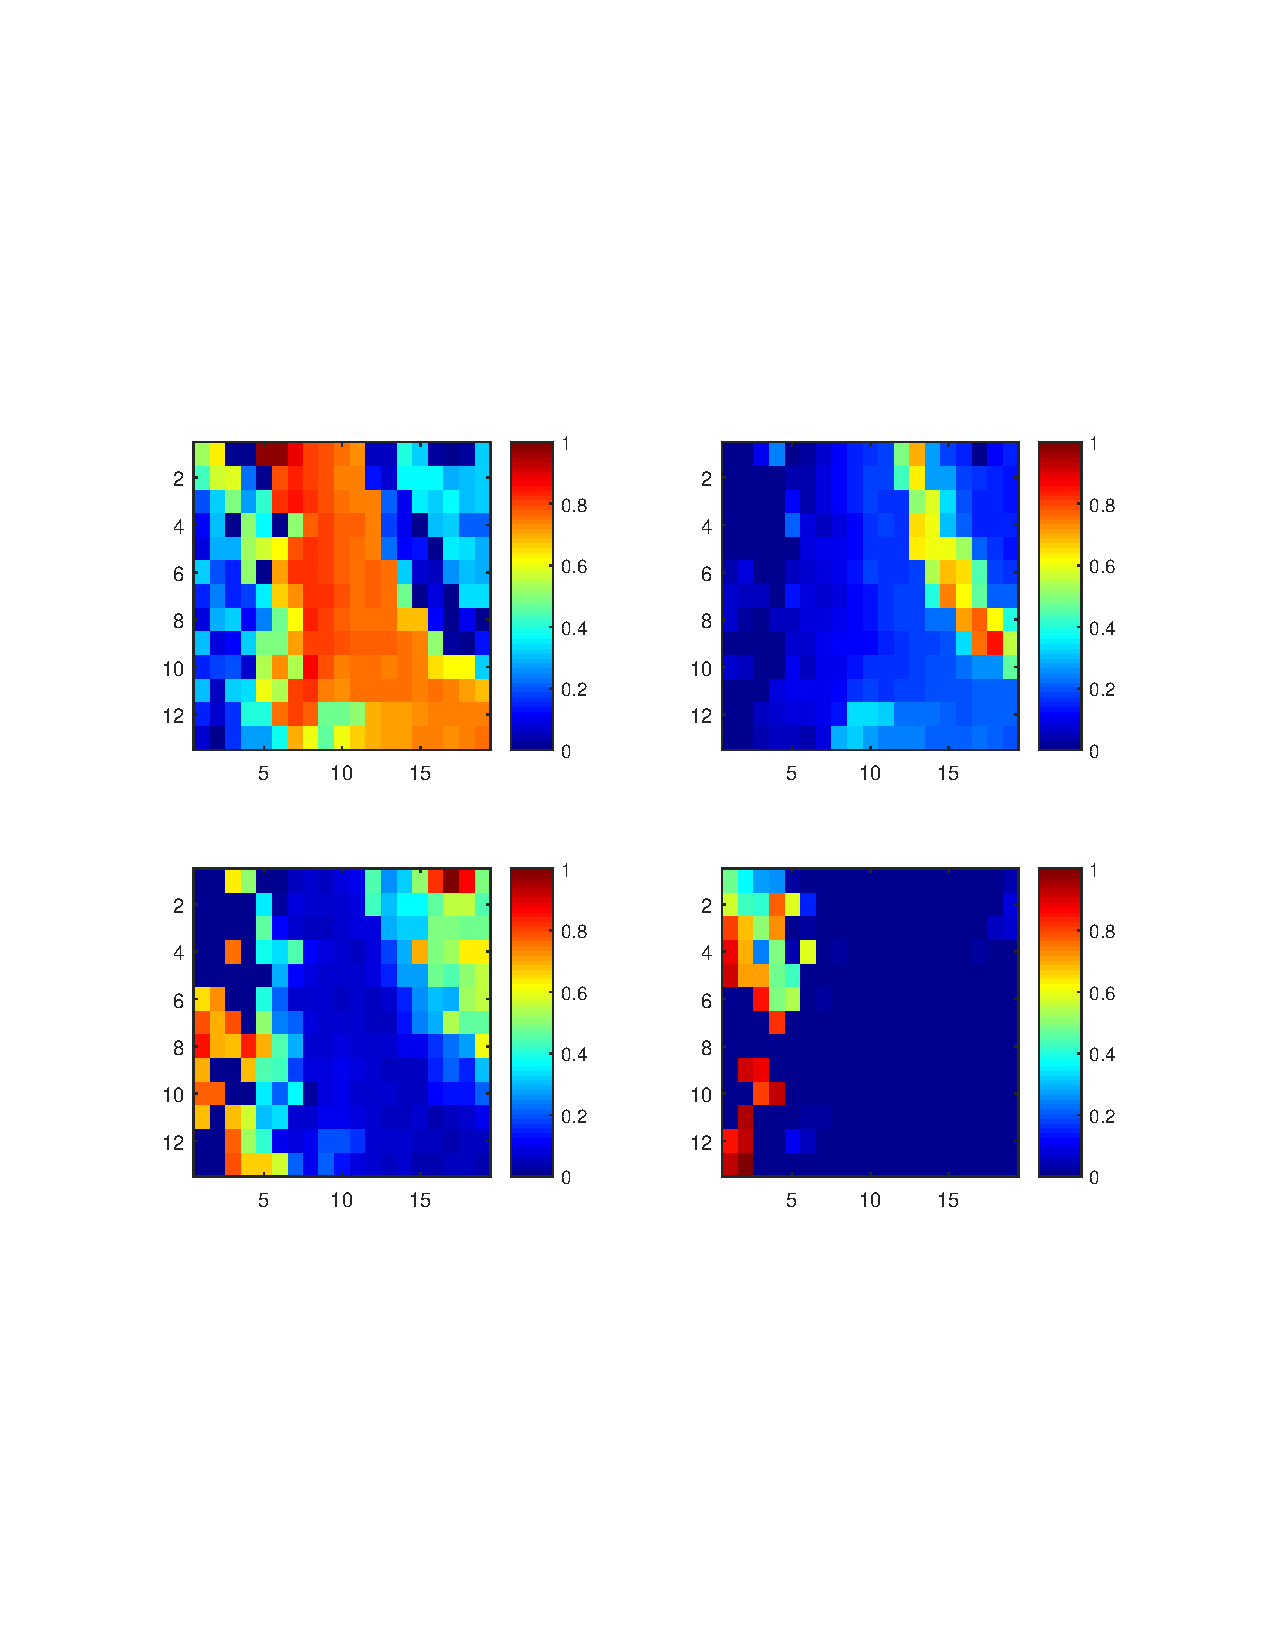
\includegraphics[width=0.99\linewidth,trim=0 200 0 175 cm]{semilinMESMA.pdf}
\caption{ontmenging van de \textit{alina dataset}\cite{alina} aan de hand van het semilineaire model. Deze figuur is gemaakt met \textit{matlab}\cite{MATLAB} \label{fig:asl}}
\end{figure}

\begin{figure}
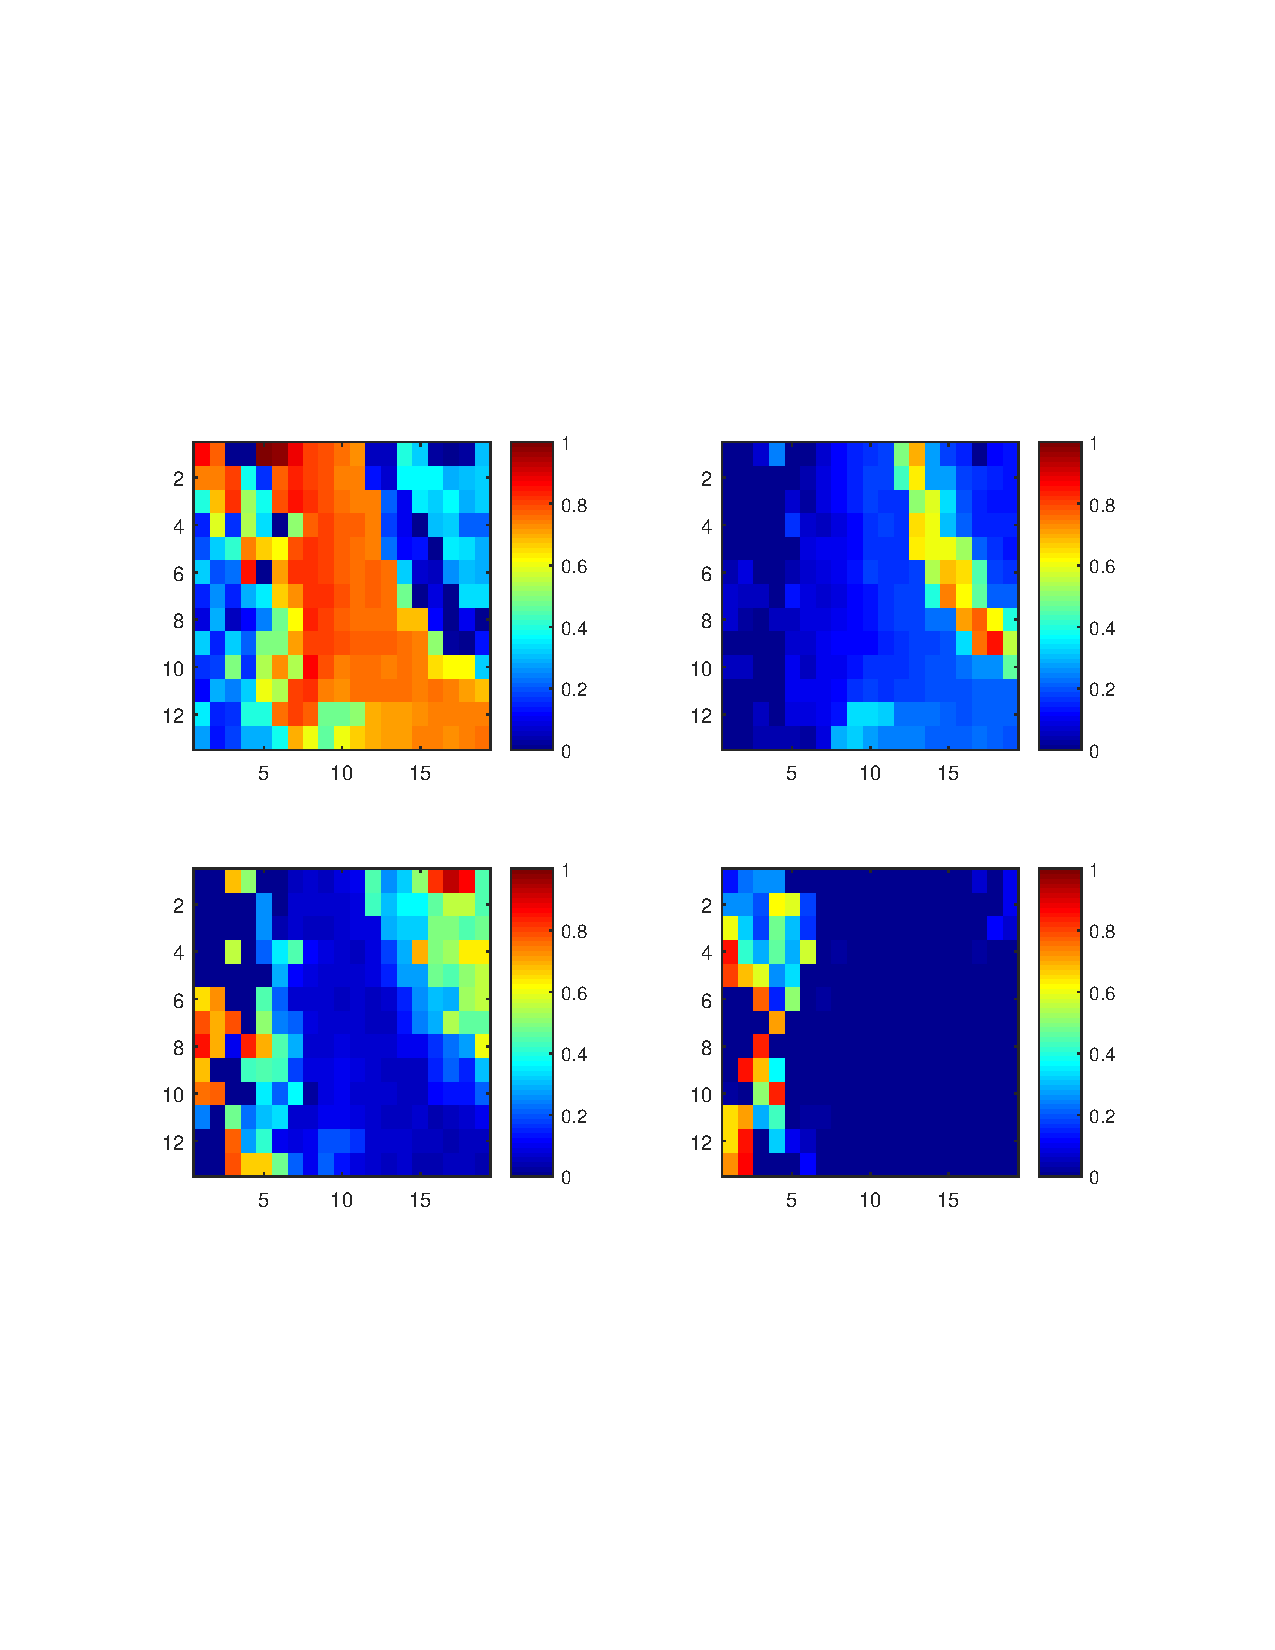
\includegraphics[width=0.99\linewidth,trim=0 200 0 175 cm]{linMESMA.pdf}
\caption{ontmenging van de \textit{alina dataset}\cite{alina} aan de hand van het lineaire model. Deze figuur is gemaakt met \textit{matlab}\cite{MATLAB} \label{fig:al}}
\end{figure}


\begin{appendices}



%\chapter{Modus van een continue dataset} \label{sec:modus}
%In de wiskunde is de modus gedefineerd als de waarde in de dataset die het vaakst voorkomt. Wanneer deze dataset continu is, zal elke waarde exact evenvaak voorkomen.Dit porbleem kunnen we oplossen door elke waarde te vervangen door een kansdichtheid rond deze waarde, en dan als modus de waarde met de grootste kansdichtheid te kiezen. Als kansdicheid rond dit pubnt nemen we een guasscurve. Het gemiddelde van deze guasscurve is evidenterwijzze de waarde zelf, en als variantie nemen we de totale variantie van onze set waarden en delen we deze door het aantal waarden. Zo is de totale variantie van de dataset gelijk aan de variantie van onze oorsponkelijke waarden.
%%TODO bewijs

\end{appendices}


\begin{flushleft}
\nocite{*}
\bibliography{biblio}{}
\bibliographystyle{amsplain}
\addcontentsline{toc}{chapter}{Bibliografie}

\end{flushleft}


\end{document}
